\documentclass[a4paper,15pt, oneside]{book}
\usepackage[italian]{babel}
\usepackage[utf8]{inputenc}
\usepackage[a4paper,top=2.5cm,bottom=2.5cm,left=2cm,right=2cm]{geometry}
\usepackage{amssymb}
\usepackage{amsthm}
\usepackage{graphics}
\usepackage{amsfonts}
\usepackage{amsmath}
\usepackage{amstext}
\usepackage{engrec}
\usepackage{rotating}
\usepackage[safe,extra]{tipa}
\usepackage{multirow}
\usepackage{hyperref}
\usepackage{enumerate}
\usepackage{braket}
\usepackage{marginnote}
\usepackage{pgfplots}
\usepackage{cancel}
\usepackage{polynom}
\usepackage{booktabs}
\usepackage{enumitem}
\usepackage{algorithm}
\usepackage{algpseudocode}
\usepackage{framed}
\usepackage{pdfpages}
\usepackage{pgfplots}
\usepackage{fancyhdr}
\usepackage{caption}
\usepackage{subcaption}
\usepackage{setspace}
\usepackage{hyperref}
\pagestyle{fancy}
\fancyhead[L,RO]{\slshape \rightmark}
\fancyfoot[C]{\thepage}

\title{Architetture Dati}
\author{Tommaso Ferrario (\href{https://github.com/TommasoFerrario18}{@TommasoFerrario18}) \\\\
Telemaco Terzi (\href{https://github.com/Tezze2001}{@Tezze2001}) \\\\
Simone Vendramini (\href{https://github.com/simone-vendramini}{@simone-vendramini})}
\date{Marzo 2024}

\pgfplotsset{compat=1.13}

\begin{document}

\maketitle
\newtheorem{teorema}{Teorema}
\newtheorem{dimostrazione}{Dimostrazione}
\newtheorem{definizione}{Definizione}
\newtheorem{esempio}{Esempio}
\newtheorem{osservazione}{Osservazione}
\newtheorem{nota}{Nota}
\newtheorem{corollario}{Corollario}
\tableofcontents
\renewcommand{\chaptermark}[1]{
    \markboth{\chaptername
        \ \thechapter.\ #1}{}}
\renewcommand{\sectionmark}[1]{\markright{\thesection.\ #1}}

\chapter*{Introduction}
\textbf{Deep Learning} is a subset of machine learning that is concerned with 
neural networks that are use to learn underlying features in data.

In general, we can define machine learning as a program that starting from the 
input and the output of a system, learns the rules that govern the system. In 
order to obtain high performance, machine learning algorithms depends heavily on 
the \textbf{representation} of the data. Representation is therefore the fundamental, 
and many artificial intelligence tasks can be solved by designing the right set of features.

The most difference between Deep ML and ML is that, the first one try to learn an
efficient representation of data and than use it to train a learn model. The latter 
one use a representation of data specified by an expert to train a learn model.

Deep Learning use neural networks with many layers of activity vectors as 
representations and learning the connection strengths between that give rise to 
these vectors by following the stochastic gradient of an objective function that
measures how well the network is performing.

So, the key ingredient of deep learning is \textbf{Depth}. There are two main 
ways to measure the depth of a model:
\begin{enumerate}
    \item in terms of depth of the graph describing how concepts are related to
        each other.
    \item in terms of number of sequential instructions that must be executed to 
        evaluate the architecture. This can be influenced by the choice of basic 
        functions used.
\end{enumerate}

One solution to the problem of feature representation is to use machine learning
not only to find the mapping between input and output, but also to find the
representation itself. This approach is called \textbf{Representation Learning}.
The goal of this task is to identify the \textit{factor of variations} that 
explain the observed data. The goal of this task is to identify the factor of 
variations that explain the observed data.

The most common example of representation learning is the use of autoencoders.

A key part of representation learning consists in the \textbf{distributed 
    representation}, which means a many to many relationship between two types
of representation:
\begin{itemize}
    \item Each concept is represented by many neurons.
    \item Each neuron participates in the representation of many concepts.
\end{itemize}

Deep learning solves this central problem in representation learning by introducing
representations that are expressed in therms of other, simpler representations.
An example is bunch of letters form words, sets of words form phrases.

\chapter{DBMS}
\section{Introduzione}
Nel percorso universitario affrontato fino a questo momento, sono state studiate
le basi di dati centralizzate, ovvero basi di dati in cui i dati sono memorizzati
in un unico luogo. L'architettura di tali strumenti è definita attraverso:
\begin{itemize}
      \item Uno o più spazi per la memorizzazione dei dati, tutti localizzati nello
            stesso luogo.
      \item Il DBMS, che è un software che consente di gestire i dati.
      \item Un'interfaccia che consente agli utenti di leggere e scrivere i dati.
\end{itemize}
\begin{definizione}[\textbf{DBMS}]
      Un \textbf{DBMS} (DataBase Management System) è un sistema software in grado
      di gestire collezioni di dati che siano:
      \begin{itemize}
            \item \textbf{Grandi}: di dimensioni molto maggiori rispetto alla memoria
                  centrale dei sistemi di calcolo utilizzati.
            \item \textbf{Persistenti}: i dati devono essere memorizzati su un
                  supporto di memorizzazione non volatile. Il periodo di vita dei
                  dati è indipendente dalle singole esecuzioni dei programmi che li
                  utilizzano.
            \item \textbf{Condivisi}: i dati devono essere accessibili da più utenti
                  contemporaneamente e anche da applicazioni diverse.
            \item \textbf{Affidabili}: devono essere resistenti a guasti.
      \end{itemize}
\end{definizione}
Per quanto riguarda i DBMS centralizzati, la loro architettura dati è definita
su tre livelli:
\begin{enumerate}
      \item \textbf{Schema esterno}: rappresenta ciò che vede l'utente finale,
            permette all'utente di avere viste personalizzate dei dati.
      \item \textbf{Schema concettuale} (logico): è la rappresentazione dei dati in modo
            indipendente dal DBMS. Questo schema è definito attraverso un modello
            di dati, che può essere relazionale, gerarchico, a oggetti, ecc.
      \item \textbf{Schema fisico}: questo schema rappresenta l'approccio fisico
            del sistema e quindi le modalità utilizzate da un DBMS per implementare
            le sue tabelle, le sue configurazioni, tutti i dati di cui ha bisogno
            sulla memoria fisica stessa.
\end{enumerate}
\begin{nota}
      Uno schema fisico è associato ad un solo schema concettuale (logico).
\end{nota}
I DBMS sono solitamente posizionati tra la base di dati fisica e le applicazioni
che la utilizzano. Questo permette di separare la gestione dei dati dalla
gestione delle applicazioni, permettendo di modificare le applicazioni senza
modificare i dati e viceversa.

Le principali caratteristiche di un DBMS Centralizzato sono:
\begin{itemize}
      \item Un unico schema logico, ovvero un'unica semantica.
      \item Un'unica base di dati, ovvero un unico insieme di record interrogati
            ed aggiornati da tutti gli utenti.
      \item Nessuna forma di eterogeneità concettuale.
      \item Un unico schema fisico, ovvero un'unica rappresentazione fisica dei
            dati.
      \item Nessuna distribuzione e nessuna eterogeneità fisica.
      \item Un unico linguaggio di interrogazione, quindi un'unica modalità di
            accesso e selezione dei dati di interesse.
      \item Un unico sistema di gestione, quindi un'unica modalità di accesso,
            aggiornamento e gestione delle transazioni.
      \item Un'unica modalità di ripristino a fronte di guasti.
      \item Un unico amministratore dei dati e quindi nessuna autonomia gestionale.
\end{itemize}

Visto che i dati che devono essere gestiti dai DBMS sono \textbf{grandi} e
\textbf{persistenti}, spesso più grandi della memoria centrale, allora i compiti
principali che questi sistemi devono eseguire riguardano la \textbf{memorizzazione
      fisica efficiente} delle strutture dati sulla memoria secondaria oltre alla
\textbf{scelta efficiente delle pagine} da trasferire nel buffer della memoria
centrale.

Una base di dati è una \textbf{risorsa integrata} e \textbf{condivisa} tra diverse
applicazioni. Questo rende necessario introdurre meccanismi di \textbf{autorizzazione}
e di \textbf{controllo della concorrenza} per gestire le operazioni di accesso
ai dati.

In un mondo ideale, le \textbf{transazioni} sono \textbf{corrette} se sono
\textbf{seriali}, ma questo penalizzerebbe di molto l'efficienza del sistema e
quindi si introduce il \textbf{controllo della concorrenza} per trovare un
compromesso ragionevole.

Quando gli utenti eseguono le \textbf{query} sulle basi di dati, lo fanno avendo
a disposizione lo schema logico. Questo schema però non rappresenta come sono
realmente memorizzati i dati, inoltre, le rappresentazioni logiche sono poco
efficienti in memoria secondaria. Per questo motivo, i DBMS devono
\textbf{tradurre} le query in modo da ridurre al minimo il numero di accessi
alla memoria secondaria, quindi si effettuerà un'\textbf{ottimizzazione delle query}.

Un modo per gestire l'\textbf{affidabilità} delle basi di dati è quello di utilizzare
\textbf{transizioni atomiche} e \textbf{definitive}, ovvero operazioni che
vengono eseguite completamente o non vengono eseguite affatto. Questo permette
di mantenere la consistenza dei dati anche in caso di guasti.
\section{Architettura di un DBMS}
L'architettura dietro ad un DBMS centralizzato è raffigurata nella figura \ref{fig:DBMS_architecture}
\begin{figure}[!ht]
      \centering
      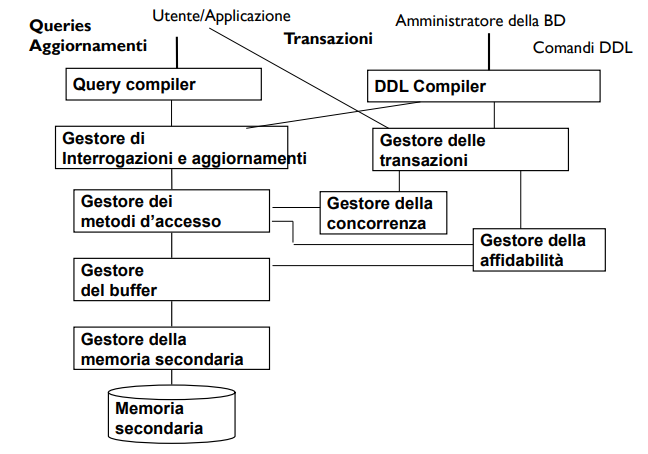
\includegraphics[width=0.7\textwidth]{./img/DBMS/Architettura.png}
      \caption{Architettura di un DBMS}
      \label{fig:DBMS_architecture}
\end{figure}
\subsection{Gestione degli accessi e delle interrogazioni}
La gestione degli accessi e delle interrogazioni inizia con la struttura del database
espressa Database administrator mediante i comandi DDL che vengono interpretati
dal DDL compiler e nel DBMS viene costruita la struttura dello schema.

A questo punto, il \textbf{Query compiler} si occupa di compilare le queries e di
passarle al \textbf{gestore delle interrogazioni}. Questo componente si occupa
dell'ottimizzazione e della frammentazione in comandi elementari per l'accesso.
In seguito, i comandi vengono passati al \textbf{gestore dei metodi di accesso},
che li trasforma in accessi alle pagine (quindi in comandi per l'accesso
alla struttura in memoria). Si passa poi al \textbf{gestore del buffer}, il quale
è responsabile della ottimizzazione. Infine, i comandi vengono inviati al
\textbf{gestore della memoria secondaria}, che si occupa tradurre i comandi in
accessi alle pagine sul disco.
\subsection{Gestione delle transazioni}
Il \textbf{gestore delle transazioni} si occupa di eseguire le transazioni e
garantire, interagendo col \textbf{gestore dell'affidabilità} e il \textbf{gestore
      della concorrenza} (scheduler), che le transazioni rispettino le proprietà
di atomicità, consistenza, isolamento e durabilità (ACID).
\section{Ottimizzazione delle interrogazioni}
La fase di ottimizzazione delle interrogazioni è suddivisa in diversi passaggi
come rappresentato in figura \ref{fig:Query_Optimization}.
\begin{figure}[!ht]
      \centering
      \includegraphics[width=0.7\textwidth]{./img/DBMS/Ottimizzazione_query.png}
      \caption{Ottimizzazione delle interrogazioni}
      \label{fig:Query_Optimization}
\end{figure}
\subsection{Fasi dell'ottimizzazione delle interrogazioni}
\begin{enumerate}
      \item Verificare che la query sia sintatticamente corretta. Per fare ciò,
            si utilizza il \textbf{Data Catalog}, che contiene le informazioni
            riguardanti la struttura dello schema.
            Questa operazione traduce la query in algebra relazionale e costruisce
            successivamente un query tree.
      \item Si trasforma un query tree in un query plan logico che viene ottimizzato
            per ridurre il suo costo di esecuzione. Per l'ottimizzazione si
            utilizza un altro database particolare è \textbf{Statistics}
            contenente statistiche sulla storia di esecuzioni precedenti delle
            interrogazioni.
      \item Si trasformano le espressioni scritte in algebra relazionale in
            espressioni che possono essere eseguite in modo efficiente. (si
            ottimizza l'espressione di algebra relazionale)
      \item Si trasforma il query plan logico in un query plan fisico, ovvero
            si mappano le operazioni dell'algebra relazionale sulle loro
            implementazioni per l'accesso alle strutture dati in memoria e si eseguono.
\end{enumerate}
\begin{nota}
      In generale l'ottimizzazione del query plan avviene anticipando il prima possibile
      le selezioni e posticipando il più possibile le join in modo da ridurre il più
      possibile la dimensione delle tabelle che sono da unire.
\end{nota}
\begin{definizione}[\textbf{Query Tree}]
      La query viene rappresentata come un albero nel quale:
      \begin{itemize}
            \item Le foglie corrispondono alle strutture dati logiche (tabelle).
            \item I nodi intermedi rappresentano operazioni algebriche:
                  \begin{itemize}
                        \item Selezione
                        \item Proiezione
                        \item Join
                        \item Prodotto cartesiano
                        \item Operazioni insiemistiche
                  \end{itemize}
      \end{itemize}
\end{definizione}
Chiaramente queste trasformazioni vengono eseguire mediante una strategia che
usa proprietà algebriche e una stima dei costi delle operazioni fondamentali per
i diversi metodi di accesso. In generale il problema di ottimizzazione delle
query è esponenziale, ma si utilizzano delle approssimazioni ragionevoli basate
su euristiche.
\section{Gestione delle transazioni}
Le transazioni sono degli insiemi di istruzioni di lettura e scrittura sulla base
di dati che godono di alcune proprietà che permettono la loro corretta esecuzione
in \textbf{ambienti concorrenti} e \textbf{non affidabili}.

Generalmente vengono identificate da un inizio begin - transaction e una fine
end - transaction e al cui interno deve essere eseguito una e una sola
volta uno dei seguenti comandi:
\begin{itemize}
      \item \textbf{commit work} per terminare correttamente
      \item \textbf{rollback work} per abortire la transazione e ripristinare lo
            stato iniziale della transazione.
\end{itemize}
Un \textbf{sistema transazionale} (OLTP) è in grado di definire ed eseguire
transazioni per un certo numero di applicazioni concorrenti.

Le transazioni godono delle proprietà \textbf{ACID}:
\begin{itemize}
      \item \textbf{Atomicità}: una transazione è un'unità indivisibile di
            esecuzione che deve essere eseguita completamente o non deve essere
            eseguita affatto.
      \item \textbf{Consistenza}: una transazione deve portare il database da uno
            stato consistente ad un altro stato consistente. Durante l'esecuzione
            di una transazione si possono avere mancanze di consistenze, l'importante
            è che al suo termine la consistenza deve essere mantenuta.
      \item \textbf{Isolamento}: le transazioni devono essere eseguite in modo
            indipendente l'una dall'altra.
      \item \textbf{Durabilità}: una transazione che ha terminato con successo
            deve essere persistente anche in caso di guasti.
\end{itemize}
Se queste proprietà non sono rispettate si possono verificare delle anomalie,
come:
\begin{itemize}
      \item \textbf{Loss updates}: due transazioni leggono lo stesso
            dato, lo modificano e lo scrivono, ma solo una delle due modifiche
            viene mantenuta.
      \item \textbf{Dirty reads}: una transazione legge un dato che è stato
            modificato da un'altra transazione che non ha ancora fatto il commit.
      \item \textbf{Non-repeatable reads}: una transazione legge due
            volte lo stesso dato e ottiene due valori diversi.
      \item \textbf{Phantom reads}: una transazione legge due volte lo stesso
            insieme di dati e ottiene due insiemi diversi.
\end{itemize}
\subsection{Gestione della concorrenza}
La gestione della concorrenza è necessaria per garantire l'isolamento delle
transazioni. Questo è necessario perché le transazioni possono essere eseguite
in modo concorrente e quindi possono accedere contemporaneamente agli stessi
dati.
\begin{definizione}[\textbf{Schedule}]
      Una sequenza di esecuzione di un insieme di transizioni è detta \textbf{schedule}.
\end{definizione}
\begin{definizione}
      Uno \textbf{schedule} si dice \textbf{seriale} se una transazione è eseguita
      per intero prima che un'altra inizi.
\end{definizione}
Si sfrutta quindi la proprietà di isolamento facendo in modo che ogni
transazione esegua come se non ci fosse concorrenza.

Si ha quindi che uno schedule è serializzabile se l'esito della sua esecuzione è
lo stesso che si avrebbe con una qualsiasi sequenza seriale delle transazioni
contenute.

Si hanno quindi diversi algoritmi per il controllo della concorrenza secondo
varie tipologie:
\begin{itemize}
      \item \textbf{Controllo basato su conflict equivalente.}
      \item \textbf{Controllo di concorrenza basato su locks:} (protocollo 2PL o two
            phase locking, shared locks e gestione dei deadlock). Il protocollo
            2PL è usato nei DBMS dove per costruzione si hanno schedule
            serializzabili usando i lock per bloccare l'accesso alla risorse da
            parte di una transazione fino a che una risorsa non sia rilasciata.
            Si hanno quindi i concetti di lock e unlock che garantiscono l'uso
            esclusivo di una risorsa e l'autorizzazione esclusiva dell'uso di una
            risorsa viene dato dal gestore delle transazioni. I lock si possono
            richiedere su tabelle, database o porzioni di tabelle.
            Inoltre, in ogni transazione, tutte le richieste di lock precedono tutte
            le richieste di unlock. L'utilizzo dei lock è trasparente rispetto alle
            transazioni, infatti si avrà un TM (transaction manager) che gestirà
            l'accesso alla risorsa tenendo traccia delle risorse già impegnate e quelle
            libere. Inoltre, il TM aggiunge le richieste di lock e unlock alle
            transazioni in automatico per preservare il comportamento serializzabile.

            Il protocollo 2PL è composto da due fasi:
            \begin{itemize}
                  \item \textbf{Fase di crescita}: in questa fase una transazione può
                        richiedere lock su una risorsa, ma non può rilasciarli.
                  \item \textbf{Fase di decrescita}: in questa fase una transazione può
                        rilasciare i lock, ma non può richiederli.
            \end{itemize}
            viene solitamente utilizzato per organizzare le transazioni in modo
            che non possano essere eseguiti unlock prima di aver preso tutti i lock.
      \item \textbf{Controllo di concorrenza basato su timestamps.}
\end{itemize}
\chapter{Basi di dati relazionali distribuite}
\begin{definizione}[\textbf{DDBMS}]
    Un \textbf{DBMS distribuito eterogeneo autonomo} è in generale una
    federazione di DBMS che collaborano per fornire accesso ai dati con livelli
    di trasparenza.
\end{definizione}
Con il termine trasparenza si intende la capacità di un sistema di
nascondere i dettagli di implementazione e di gestione dei dati, fornendo
all'utente una visione unificata e coerente del sistema, spesso nascondendo i gli
aspetti di \textbf{distribuito}, \textbf{eterogeneo} e \textbf{autonomo}.

In base a questi aspetti si definisce una classificazione dei DDBMS per ogni aspetto
e una classificazione per la combinazione dei tre aspetti.

La più importante classificazione che riguarda i $3$ aspetti è:
\begin{itemize}
    \item \textbf{DBMS Distribuiti Omogenei} (DDBMS): C'è distribuzione ma
          nessuna eterogeneità e nessuna autonomia.
    \item \textbf{DBMS Distribuito Eterogeneo}: In questa fase vederemo il
          problema dell'integrazione dei dati.
    \item \textbf{Multi Database MS}: Sistemi totalmente autonomi.
\end{itemize}

\paragraph{Autonomia} L'\textbf{autonomia} di un'architettura dati distribuita fa riferimento
al grado di \textbf{indipendenza} tra i nodi. Possiamo distinguere diversi livelli di autonomia:
\begin{itemize}
    \item \textbf{Autonomia di progetto}: ogni nodo ha un proprio modello dei
          dati e di gestione delle transizioni.
    \item \textbf{Autonomia di condivisione}: ogni nodo sceglie la porzione di
          dati da condividere con gli altri nodi.
    \item \textbf{Autonomia di esecuzione}: ogni nodo sceglie in che modo eseguire
          le transazioni che gli vengono inviate.
\end{itemize}
Partendo da questa classificazione possiamo definire diversi tipi di DBMS autonomi:
\begin{itemize}
    \item \textbf{DBMS Strettamente integrati}: in questo caso non c'è nessuna
          autonomia, si ha un unico \textbf{data manager} (DM) centralizzato
          responsabile delle transazioni applicative. I data
          manager locali non operano in maniera autonoma.
    \item \textbf{DBMS Semi - autonomi}: ogni DM è autonomo ma partecipa
          alle transazioni globali. Una parte dei dati è condivisa e richiedono
          modifiche architetturali per poter far parte della federazione.
    \item \textbf{DBMS Totalmente autonomi} (peer - to - peer): ogni DBMS lavora in
          completa autonomia ed è inconsapevole dell'esistenza degli altri.
\end{itemize}

\paragraph{Distribuzione} La \textbf{distribuzione} dei dati può avvenire in diversi
modi:
\begin{itemize}
    \item \textbf{Distribuzione client - server}: i dati sono distribuiti su più server
          e i client accedono ai dati attraverso le richieste fatte ai server.
          I server forniscono la gestione dei dati, mentre i client forniscono
          l'applicativo e la presentazione.
    \item \textbf{Distribuzione peer - to - peer}: i dati sono distribuiti su più nodi
          e ogni nodo può essere sia client che server. Ogni nodo è autonomo
          e può eseguire transazioni locali.
    \item \textbf{Nessuna distribuzione}: i dati sono centralizzati
\end{itemize}

\paragraph{Eterogeneità} L'\textbf{eterogeneità} si riferisce alla diversità dei DBMS
che compongono la federazione. Questa diversità può essere di diversi tipi:
\begin{itemize}
    \item \textbf{Linguaggio di interrogazione}: i DBMS possono utilizzare
          linguaggi di interrogazione diversi.
    \item \textbf{Modello dei dati}: i DBMS possono utilizzare modelli di dati
          diversi.
    \item \textbf{Sistema di gestione delle transazioni}: i DBMS possono utilizzare
          sistemi di gestione delle transazioni diversi.
    \item \textbf{Schema concettuale e logico}: i DBMS possono avere schemi concettuali
          diversi.
\end{itemize}

Per le architetture eterogenee dobbiamo occuparci di aggiungere un gestore delle
transazioni (TM) che si occupi di mappare una query distribuita sui singoli DBMS
e che si occupi della parte di \textbf{concurrency control} e \textbf{recovery}.


\section{DDBMS}
% TODO: borderline la definizione vincolata solo all'omogeneo
Vogliamo ora approfondire il concetto di \textbf{DDBMS}. Un DDBMS è un DBMS
distribuito omogeneo, ovvero un sistema in cui i dati sono distribuiti su più
nodi ma tutti i nodi utilizzano lo stesso DBMS.

Per ogni DBMS distribuito si hanno due tipologie architetture:
\begin{itemize}
    \item Architettura dati: come gestire i dati
    \item Architettura funzionale, ovvero l'insieme di tecnologie per l'implementazione
          dell'architettura dati (vedi figura \ref{fig:sharedNothing}):
          \begin{itemize}
              \item \textbf{Shared-everything}: dove il database management system e il
                    disco sono in un unico nodo.
              \item \textbf{Shared-disk}: dove diversi DBMS agiscono sugli stessi dati. I
                    vari DBMS accedono ai dati secondo una certa regolazione.
                    Viene distribuito il carico ma si hanno problemi di concorrenza e
                    hanno grandi problemi di scalabilità e costo economico
              \item \textbf{Shared-nothing}: dove ogni DBMS ha il suo disco. È molto
                    scalabile e, a patto di gestire la complessità, posso aggiungere nodi
                    in modo illimitato.
          \end{itemize}
\end{itemize}

\begin{figure}[ht]
    \centering
    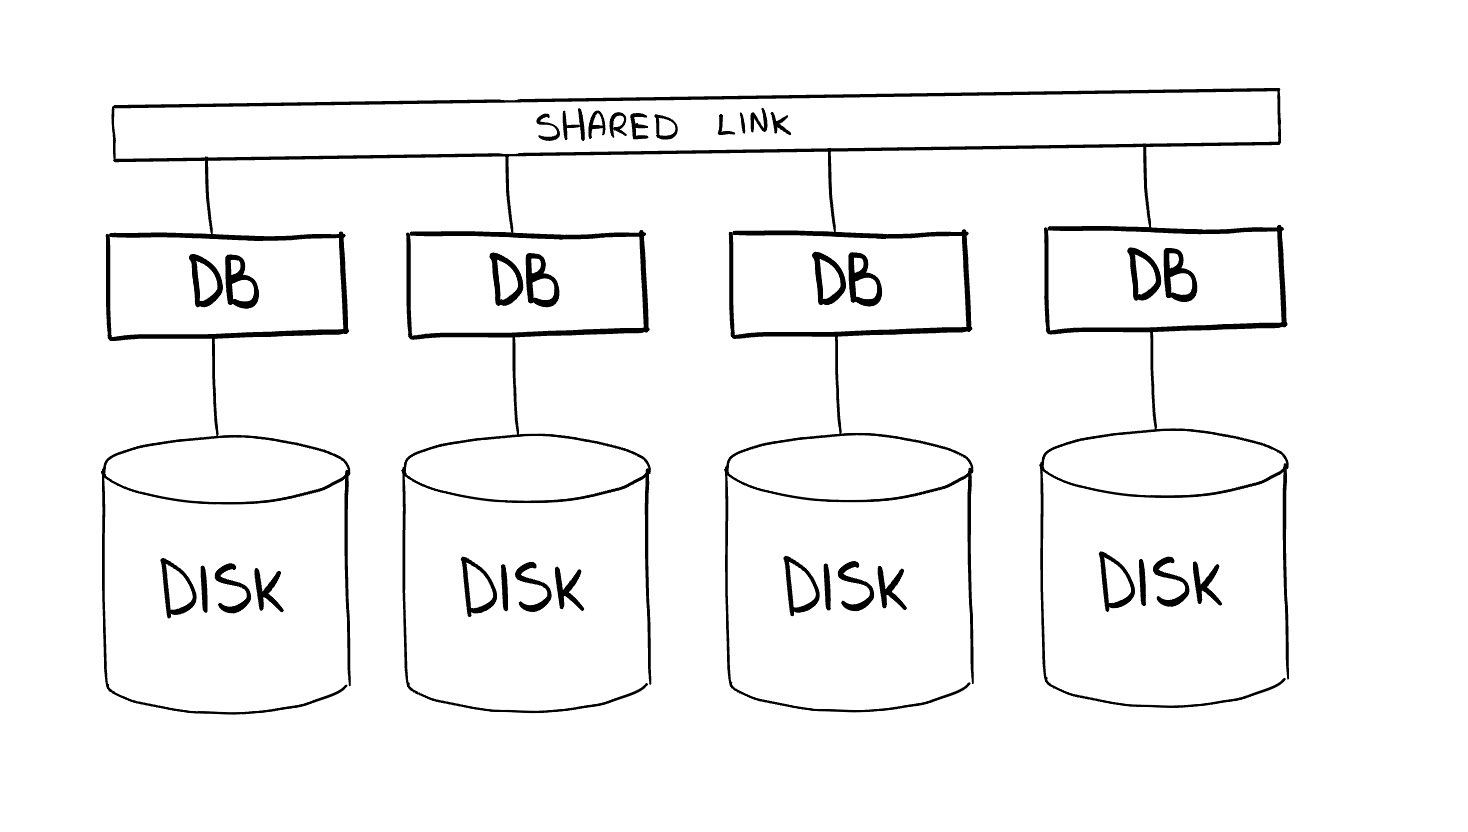
\includegraphics[width=0.60\textwidth]{img/SharedNothing.jpg}
    \caption{Architettura shared-nothing}
    \label{fig:sharedNothing}
\end{figure}

Non avendo il concetto di eterogeneità si mantiene lo stesso schema di un DBMS
centralizzato, distribuendo i dati. Questo comporta la necessità di aggiungere
uno schema logico locale tra lo schema logico e quello fisico. Non si avrà più
un solo schema logico e un unisco schema fisico, ma tanti schemi logici locali e
fisici locali (ad ogni logico corrisponde un fisico).

I vari schemi logici locali si interfacciano con uno schema logico globale,
tali schemi non sono altro che delle viste dello schema logico globale. Questa
organizzazione tra schemi logici locali e schema logico globale è la cosiddetta
organizzazione \textbf{LAV} (Local As View). L'applicazione interroga
lo schema logico globale e saranno varie a mappare le query distribuite suglis gli schemi
logici locali.

% TODO: inserisci immagine dello schema logico

Per la gestione delle query distribuite serve una cooperazione o un'orchestrazione
dei singoli DBMS che fanno parte della federazione, sopprattutto per quanto riguarda
il query processing e la gestione delle transazioni. Più precisamente si può avere
una gestione centralizzata (che può essere gerarchica) oppure distribuita con
un'assegnazione statica o dinamica dei ruoli. La determinizzazione delle modalità
si effettuerà attraverso dei protocolli.

Nella fase di \textbf{progettazione} di un \textbf{DDBMS} si hanno delle differenze rispetto alla
progettazione di un DBMS centralizzato. Si hanno cinque fasi:
\begin{enumerate}
    \item Analisi dei requisiti
    \item Progettazione concettuale
    \item Progettazione della distribuzione, per capire dove mettere i dati
    \item Progettazione logica locale per ciascun nodo, che traduce dallo schema concettuale
          globale allo schema logico locale solo alcuni concetti
    \item Progettazione fisica locale per ciascun nodo
\end{enumerate}

Per quanto riguarda DBMS DEA (distribuiti eterogenei e autonomi) dal momento che
sono composti da DBMS eterogenei allora si introduce il concetto di \textbf{portabilità},
ovvero la capacità di eseguire le stesse applicazioni DB (SW per ottenere i dati dal DB)
in ambienti runtime diversi. Questo viene facilitato dagli standard dei linguaggi
di query del DB.
Inoltre, viene aggiunto anche il concetto di \textbf{interoperabilità}, ovvero
la capacità di eseguire applicazioni che coinvolgono contemporaneamente sistemi
diversi ed eterogenei. A tal fine sono si introducono dei \textbf{middleware}, tra cui \textbf{ODBC} che si occupa dell'accesso a dati
di diversi vendor. \textbf{ODBC}, a livello architetturale, si pone sopra il DBMS e da
un'immagine indipendente da ciò che c'è sotto, trasformando tutto in una sorta
di SQL standard. Si hanno anche dei protocolli, come \textbf{X-Open Distributed
    Transaction Processing} (DTP) che consentono di eseguire delle transazioni secondo
una logica diversa. Questo protocollo stabilisce una serie di API che vengono
implementate da ogni singolo DBMS per offrire una connettività standard.

Il protocollo funziona sia se si ha che fare con omogeneità che con eterogeneità dei DDBMS.


% ! da spostare
Si hanno altri approcci:
\begin{itemize}
    \item \textbf{Basi dati parallele}, con incremento delle prestazione
          mediante parallelismo sia di storage devices che di processore
          (scalabilità orizzontale).
    \item \textbf{Basi dati replicate} dove si ha la replicazione della stessa
          informazione su diversi server per motivi di performance. Importanti
          per i temi della consistenza e della sicurezza
    \item \textbf{Data warehouses}, ovvero DBMS centralizzati, risultato
          dell'integrazione di fonti eterogenee, dedicati nel dettaglio alla
          gestione di dati per il supporto alle decisioni. Prevede la
          cristallizzazione dei dati, acquisiti da varie sorgenti, creando un
          nuovo schema con la memorizzazione dei dati in formato nuovo
          (solitamente relazionale). Non usa un approccio LAV.
\end{itemize}

\subsection{Vantaggi dei DDBMS}
I \textbf{DDBMS} hanno notevoli \textbf{vantaggi}:
\begin{itemize}
    \item \textbf{Località}: i dati sono vicino alle applicazioni che li
          utilizzano più frequentemente. Questo riduce i tempi per l'esecuzione
          delle operazioni. Il paradigma è spostare i dati verso le
          applicazioni, le partizioni dei dati corrispondono spesso a delle
          partizioni naturali delle applicazioni e degli utenti. Le
          distribuzioni dei dati spesso sono flessibili: è possibile spostare un
          intera tabella così come è possibile spostarne solo un sottoinsieme
          o replicarla.
    \item \textbf{Modularità} le modifiche alle applicazioni e ai dati possono
          essere effettuate a basso costo. Si ha una distribuzione dei dati incrementale e
          progressiva, infatti la configurazione si adatta alle esigenze delle applicazioni.
    \item \textbf{Resistenza ai guasti}: grazie alla replicazione dei dati si ha
          ridondanza (fail soft). Ovviamente la ridondanza funziona in rete quindi
          si introduce fragilità per la comunicazione in rete.
    \item \textbf{Prestazioni ed Efficienza}: distribuendo un database su più
          nodi, ogni nodo gestisce un DB di dimensioni ridotte. Questo
          significa che i singoli DB sono più facili da gestire e ottimizzare
          localmente e, in particolare, ogni nodo può adottare delle
          ottimizzazioni personalizzate. Il carico inoltre viene distribuito
          sui nodi che permette di avere parallelismi tra le transazioni che fanno
          parte della stessa transazione distribuita.
          Tutto ciò però richiede chiaramente un coordinamento tra i
          nodi e aumenta il traffico di rete che può rivelarsi un collo di
          bottiglia per le prestazioni.
\end{itemize}

\subsection{Differenze rispetto ai DBMS}
Si ha un \textbf{Indipendenza locale e cooperazione tra server}, ogni server
mantiene ha la sua applicazione, si hanno interazioni tra i vari server per la
loro cooperazione, la cooperazione può avvenire per gestire due cose:
\begin{itemize}
    \item \textbf{interrogazioni}: sia query provenienti dalle applicazioni e
          i risultati provenienti dal server
    \item \textbf{transazioni}: richieste di transazioni dalle applicazioni  e
          dati di controllo per il coordinamento dello stato delle transazioni.
\end{itemize}
Il problema è l'ottimizzazione che è limitata per via della rete e l'obiettivo
sarà quello di distribuire i dati per avere più transazioni possibili in locale.

Si hanno anche le seguenti funzionalità specifiche:
\begin{itemize}
    \item \textbf{Trasmissione} di query, transizioni, frammenti di db e dati
          di controllo tra i nodi.
    \item \textbf{Frammentazione, replicazione e trasparenza} fattori legati
          alla natura distribuita dei dati.
    \item un query processor e un query plan per la previsione di una
          strategia globale accanto a strategie per le query locali. Si gestisce
          il passaggio tra schema logico globale e quelli locali. Chi esegue
          la query lo fa senza pensare alla frammentazione dei dati
    \item \textbf{Controllo di concorrenza} tramite algoritmi distribuiti, fondamentale
          per gli accessi in scrittura.
    \item \textbf{Strategie di recovery} e \textbf{gestione dei guasti}, sia
          in merito alla rete, sia all'hardware stesso.
\end{itemize}

\subsection{Frammentazione}
\begin{definizione}[\textbf{Frammentazione}]
    Si definisce \textbf{frammentazione} come la possibilità di allocare porzioni
    diverse del database su nodi diversi.
\end{definizione}

Esistono due tipi di frammentazione:
\begin{itemize}
    \item \textbf{Frammentazione orizzontale}: si prende una tabella e la si
          frammenta in base alle righe. Si mantiene inalterato lo schema in
          quanto si ottengono solo delle tabelle più piccole. Per spezzare si
          usa una select che selezioni ogni volta un certo blocco di tabella.
          (Ex: vengono separati i dottori nati a Milano da quelli nati a Napoli,
          alla fine si effettua la union per ricostruire la tabella originale)
    \item \textbf{Frammentazione verticale}: si prende una tabella e la si frammenta
          in base alle colonne. In ogni nuova tabella però la prima colonna
          deve essere uguale alla prima della tabella originale (ovvero dove si
          ha la chiave primaria), questo per garantire che si possa ricomporre
          la tabella originale con operazioni di join e garantire la
          trasparenza. Anche in questo caso uso una select che selezioni ogni
          volta un certo numero di colonne da mettere nella nuova tabella.
          (Ex: si dividono gli attributi della tabella e si fa la join in fase di
          ricostruzione)
\end{itemize}
Quando si usa la frammentazione bisogna garantire le seguenti regole:
\begin{itemize}
    \item \textbf{Completezza}: ogni record della relazione R di partenza
          deve poter essere ritrovato in almeno uno dei frammenti
    \item \textbf{Ricostruibilità}: la relazione R di partenza deve poter essere
          ricostruita senza perdita di informazione a partire dai frammenti
    \item \textbf{Disgiunzione}: ogni record della relazione R deve essere
          rappresentato in uno solo dei frammenti
    \item \textbf{Replicazione}: l'opposto della disgiunzione
\end{itemize}
\subsection{Replicazione}

\begin{definizione}[\textbf{Replicazione}]
    Si definisce \textbf{replicazione} come la possibilità di allocare stesse
    porzioni del database su nodi diversi.
\end{definizione}

Si hanno diversi aspetti positivi per l'accesso in lettura, come il miglioramento
delle prestazioni in quanto consente la coesistenza di applicazioni con requisiti
operazionali diversi sugli stessi dati e aumenta la località dei dati usati da
ogni applicazioni. Nel momento in cui si ha l'accesso in scrittura si hanno però
diversi aspetti negativi. Si hanno diverse complicazioni architetturali, tra cui
la gestione della transazioni e l'update di copie multiple, che devono essere
tutte aggiornate. Inoltre bisogna studiare dal punto di vista progettuale cosa
replicare, quanto replicare, dove allocare le copie e le politiche per gestirle.

In merito all'allocazione studiamo anche gli schemi di allocazione. Ogni
frammento può essere allocato su un nodo diverso. Lo schema globale quindi
è solo virtuale e lo schema di allocazione definisce il mapping tra un frammento
e un nodo. Si ha quindi una tabella, un catalogo, che ci da informazioni sul
partizionamento, associando ogni frammento al nodo in cui è allocato.
\subsection{Trasparenza}

\begin{definizione}[\textbf{Trasparenza}]
    Si definisce \textbf{trasparenza} come la possibilità per l'applicazione di
    accedere ai dati senza sapere dove sono allocati.
\end{definizione}

Con la trasparenza si ha la separazione della semantica di alto livello dalle
modalità di frammentazione e allocazione. Si separa quindi la logica applicativa
dalla logica dei dati ma per farlo serve uno strato software che gestisca la
traduzione dallo schema unico ai sottoschemi, comportando un aumento di
complessità del sistema e una perdita di prestazioni.
Le applicazioni (transazioni, interrogazioni) non devono essere modificate a
seguito di cambiamenti nella definizione e organizzazione dei dati e si hanno
due tipi di trasparenza, che si applicano agli schemi ANSI-SPARC nel
modello distribuito:
\begin{enumerate}
    \item \textbf{Trasparenza logica} (o indipendenza logica), ovvero
          indipendenza dell'applicazione da modifiche dello schema logico.
          Un'applicazione che usa un frammento non viene modificata se vengono
          modificati altri frammenti.
    \item \textbf{Trasparenza fisica} (o indipendenza fisica), ovvero
          indipendenza dell'applicazione da modifiche dello schema fisico
\end{enumerate}

Frammentazione e allocazione sono tra lo schema logico globale e ogni schema
logico locale. Si hanno quindi tre livelli di trasparenza:
\begin{itemize}
    % TODO: immagini sull'effetto della trasparenza nelle  query
    \item \textbf{Trasparenza di frammentazione}, che permette di ignorare
          l'esistenza dei frammenti ed è lo scenario migliore per la
          programmazione applicativa. Il sistema si occupa di convertire query
          globali in locali e relazioni in sotto-relazioni. La scomposizione
          delle query per ogni sotto-relazione è detta query rewriting.
    \item \textbf{Trasparenza di replicazione/allocazione}, dove l'applicazione
          è consapevole dei frammenti ma non dei nodi in cui si trovano. In questo
          caso la query è già spezzata in quanto si sa di avere a che fare con un
          sistema frammentato.
    \item \textbf{Trasparenza di linguaggio}, dove l'applicazione specifica
          sia i frammenti che i nodi, nodi che possono offrire interfacce che
          non sono SQL standard. Tuttavia l'applicazione sarà scritta in SQL
          standard a prescindere dai linguaggi locali dei nodi. Le query
          vengono quindi tradotte ottimizzatone di query. Questo è il livello
          di trasparenza più basso.
\end{itemize}
% ! da spostare
\section{DBMS distribuito}
Esistono diverse architetture di DBMS distribuiti alcune delle quali sono
riportate in figura \ref{fig:DBMS_distributed_architecture}.
\begin{figure}
    \centering
    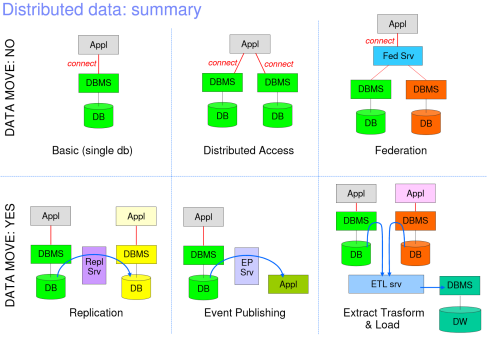
\includegraphics[width=0.7\textwidth]{./img/DBMS/DBMS_distributed_architecture.png}
    \caption{Architetture di DBMS distribuiti}
    \label{fig:DBMS_distributed_architecture}
\end{figure}

\section{Gestione delle query distribuite}
In un DBMS distribuito, a differenza dei DBMS centralizzati, le query vengono ottimizzate
in modo diverso. In particolare, si hanno le seguenti fasi:
\begin{itemize}
    \item \textbf{Query decomposition}: la query distribuita viene decomposta in
          sottoquery che possono essere eseguite in modo indipendente. Questa
          fase tiene conto dello schema logico globale e non considera la
          distribuzione dei dati. Usa delle tecniche di ottimizzazione algebrica
          come quelle usate nei DBMS centralizzati.
          In output a questa fase si ha un \textbf{query tree globale} che non tiene
          conto dei costi di comunicazione.
    \item \textbf{Data Location}: in questa fase si considera la distribuzione
          dei frammenti. Si ottimizzano le operazioni rispetto alla
          frammentazione utilizzando tecniche di riduzione. In output si ha una
          \textbf{query efficiente sui frammenti} ma non ottimizzata.
    \item \textbf{Global optimization}: in questa fase si ottimizza la query
          rispetto ai costi di comunicazione, aggiungendo agli operatori
          algebrici quelli per la comunicazione. L'obiettivo è quello di
          trovare il piano di esecuzione che minimizza il costo totale, ovvero
          l'ordine migliore delle operazioni nella query fragment. Le
          decisioni più importanti riguardano le operazioni di join perché
          non si possono trasferire gli indici e quindi è l'operazione più lenta
          (scelta se usare un join o semi-join) (Si ottimizza il costo di comunicazione).
    \item \textbf{Local optimization}: in questa fase si ottimizza il piano di
          esecuzione per ogni singolo nodo (si ottimizza indipendentemente il query fragment
          usando le ottimizzazioni centralizzate).
\end{itemize}
Gli obiettivi dell'ottimizzazione sono ridurre il costo totale, ovvero la somma
dei costi di operazioni locali come input e output, e il costo di comunicazione.
Oltre a ciò, si vuole ridurre il response time, ovvero la somma dei costi tenendo
conto del parallelismo.

% TODO: aggiungere l'immagine dello schema dell'ottimizzazione
% TODO: aggiungere l'esempio nelle slide

Il costo principale nelle basi di dati è il \textbf{costo totale} che è dipendente
dai \textbf{costi delle operazioni} (I/O e CPU) e dal costo di \textbf{costo di comunicazione}.
\begin{equation*}
    \text{costo totale} = \textbf{costo operazioni} + \text{costo di comunicazione}
\end{equation*}

Se si sommano tutti i costi di tutte le operazioni eseguite nella query distribuita,
tenendo conto del parallelismo, si ottiene il \textbf{response time}.

Nel caso distribuito il \textbf{costo di comunicazione} è quello più significativo rispetto
ai \textbf{costi delle operazioni}. Per calcolare i costi di comunicazione si
può seguire la seguente formula.
\begin{equation*}
    \text{Costo comunicazione} = \text{C\_{MSG}} \cdot \#\ msgs  + \text{C\_{TR}} \cdot \#bytes
\end{equation*}
dove:
\begin{itemize}
    \item \textbf{$C\_{MSG}$} è il costo di trasmissione di un messaggio
    \item \textbf{$C_{TR}$} è il costo di trasmissione fisso di un byte dipendente dalla topologia
    \item \textbf{$\#\ msgs$} è il numero di messaggi
    \item \textbf{$\#bytes$} è il numero di byte
\end{itemize}

Per calcolare il \textbf{tempo di risposta} (response time), a differenza del
costo totale, i costi delle operazioni in parallelo non si sommano,
ottenendo la seguente formula:
\begin{equation*}
    \text{Tempo di risposta} = C\_{MSG} \cdot seq\_\#msgs + C_{TR} \cdot seq\_\#bytes
\end{equation*}
dove $seq\_\#msgs$ è il massimo numero di messaggi che devono essere comunicati
in modo sequenziale.

Naturalmente, il costo più importante deve essere valutato in base a alla
situazione in cui mi trovo. Chiaramente se si lavora in una grande rete
geografica, il costo di comunicazione sarà molto più alto rispetto al costo di
esecuzione locale. Viceversa nelle reti locali, il costo di comunicazione sarà
molto più basso rispetto al costo di esecuzione locale. Ovviamente possiamo calcolare
il costo totale assegnando dei pesi ai singoli costi.

Possiamo essere interessati a:
\begin{itemize}
    \item \textbf{Minimizzazione tempo di risposta}: più parallelismo può portare ad
          aumento del costo totale (maggiore numero di trasmissioni e
          processing locale)
    \item \textbf{Minimizzazione costo totale}: somma dei costi senza tener conto del
          parallelismo: utilizza meglio le risorse e aumento del throughput (con
          peggioramento del response time in generale)
\end{itemize}

\subsection{Operazione di join}
Dato che nei join quando si trasferiscono i dati non è possibile passare gli indici,
le operazioni di join sono quelle più costose dal punto di vista computazionale.
Per questo motivo, l'operazione di \textbf{semijoin} può essere in alcune circostanze
un'alternativa più efficiente rispetto al join.
\begin{definizione}[\textbf{Semijoin}]
    Dati due insiemi $R$ e $S$, il semijoin di $R$ e $S$ è definito come:
    \begin{equation*}
        R \text{semijoin}_A S \equiv \pi_{R^\ast}(R \, \text{join}_A \, S)
    \end{equation*}
    dove $R^\ast$ è l'insieme delle colonne di $R$. Il semijoin è la proiezione
    sugli attributi di $R$ del join di $R$ e $S$.
\end{definizione}
\begin{nota}
    Il semijoin non è commutativo.
\end{nota}
Chiaramente l'uso del semi - join è conveniente se il costo del suo calcolo e
del trasferimento del risultato sono inferiori al costo di trasferimento
dell'intera relazione del costo del join intero.

In generale, l'uso del semijoin è più conveniente se il costo del suo calcolo e
del trasferimento del risultato è inferiore al consto del trasferimento
dell'intera relazione e del costo del join intero.

\section{Controllo della concorrenza}
Fino a questo momento abbiamo considerato le interrogazioni più semplici. Vogliamo
ora analizzare la gestione delle scritture sui database distribuiti. In particolare,
possiamo classificare le transazioni in due categorie:
\begin{itemize}
    \item \textbf{Dirette a un unico server remoto}: in questo caso il controllo
          della concorrenza è simile a quello dei DBMS centralizzati. Dobbiamo
          distinguere tra due tipi di transazioni:
          \begin{itemize}
              \item \textbf{Remote request}: ovvero transazioni di sola lettura
              \item \textbf{Remote transaction}: ovvero transazioni di lettura e scrittura.
          \end{itemize}
    \item \textbf{Dirette a un numero arbitrario di server}: in questo caso il
          controllo della concorrenza è più complesso. In questo caso la
          classificazione si divide in:
          \begin{itemize}
              \item \textbf{Distributed requests}: operazioni read - only
                    arbitrarie nelle quali ogni singola operazione SQL si può riferire
                    a qualunque insieme dei server. Richiede un ottimizzatore distribuito.
              \item \textbf{Distributed transactions}: numero arbitrario di
                    operazioni SQL, ogni operazione è diretta ad un unico server.
                    Le transazione possono modificare più di un database. Richiede
                    un protocollo transazionale di coordinamento distribuito (two
                    - phase commit).
          \end{itemize}
\end{itemize}

La \textbf{distribuzione} non ha conseguenze su \textbf{consistenza} e \textbf{durabilità} in quanto la
consistenza non dipende dalla distribuzione poiché i vincoli descrivono solo
proprietà logiche dello schema. Mentre, la durabilità è garantita localmente da
ogni sistema.

È invece necessario rivedere alcuni componenti dell'architettura in merito a
\textit{isolamento} tramite concurrency control e ad \textit{atomicità} tramite
reliability control e recovery manager.

L'idea alla base del controllo della concorrenza è che ogni transizione $t_i$
possa essere suddivisa in $t_{ij}$ transazioni che saranno eseguite sul nodo $j$.
Ogni sotto-transazione viene schedulata in modo indipendente dai server di
ciascun nodo. La schedule globale dipende quindi dalle schedules locali su ogni nodo.

In questo modo lo schedule globale andrà a dipendere dallo schedule locale di
ciascun nodo. Inoltre in questo caso, seppur localmente le transazioni sembrino
serializzabili, si crea la possibilità di avere conflitto a livello globale.
\subsection{ROWA}
Nel caso di database non è replicato e ogni schedule locale è serializzabile
allora lo schedule globale è serializzabile se gli ordini di serializzazione
sono gli stessi per tutti i nodi, ovvero se il flusso delle transazioni è lo
stesso per tutti i nodi.

Quando si aggiunge la replicazione dei dati le cose cambiano. Nello specifico
possiamo violare la mutua consistenza dei database locali per la quale tutte le
copie devono avere lo stesso valore al termine della transazione. Abbiamo quindi
bisogno di un protocollo di controllo delle repliche.

Un protocollo è il \textbf{ROWA} (\textbf{Read Once Write All}). Questo
protocollo mappa le operazioni di lettura su una qualunque delle copie, mentre
le operazioni di scrittura vengono mappate su tutte le copie. Di fatto, finché
non sono accertate tutte le write su tutte le copie, la transazione non continua.

Questo protocollo garantisce la consistenza dei dati ma a scapito chiaramente delle
performance. Questa condizione può essere rilassata con dei protocolli asincroni
più efficienti.

Nel distribuito il 2PL  non funziona più.

\subsection{Two Phase Locking}
Nella progettazione della base di dati bisogna considerare diverse informazioni:
\begin{itemize}
    \item Topologia della rappresentazione.
    \item Tipologie di query distribuite.
    \item Stime o statistiche su query distribuite.
\end{itemize}

In aggiunta dobbiamo considerare i problemi di scrittura e quindi problemi di
concorrenza. Dobbiamo costruire una serie di protocolli che ci permettono di
risolvere questi problemi, nel sistema centralizzato un metodo è quello di usare
2PL, il quale sfrutta i lock (accesso esclusivo) sulle risorse (tabelle, blocchi
di pagina o righe) per eseguire le transazioni.

Vediamo ora come possiamo risolvere questo problema nel caso distribuito. Sul
singolo nodo le transazioni verranno gestite come nel caso centralizzato. Questo
però non risolve i problemi di deadlock distribuiti. Per risolvere questo problema
bisogna avere una vista globale del sistema, in aggiunta tutto si complica
aggiungendo le repliche.

Con l'aggiunta di quest'ultime si introduce il problema sull'atomicità, perché
bisogna assicurarsi che una scrittura venga replicata su tutti i nodi, e che sia
fatta in modo efficiente. Una soluzione a questo problema è il protocollo ROWA,
il quale consiste nello scrivere su tutte le repliche e poi segnalano quando
hanno finito, in questo modo posso leggere da qualsiasi nodo. Questo approccio
comporta rallentamenti dal momento che le repliche sono dislocate geograficamente.

Si può estendere 2PL al caso distribuito introducendo un coordinatore delle
transaction centrale e un lock manager per ogni nodo. Uno di questi lock manager
viene eletto come coordinatore e si occupa di gestire i lock tra i vari nodi.

La strategia in questo caso è quella che il Transaction Manager (TM) lancia la
transazione e utilizza un lock manager centrale che gestisce i lock tra tutti i
nodi. Il lock manager centrale la esegue utilizzando 2 phase locking. A questo
punto il transaction manager comunica ai data processor di eseguire le operazioni.
Una volta che il data processor ha finito, comunica al lock manager centrale che
ha finito e il lock manager centrale comunica al transaction manager che può fare
commit.

Questo approccio vuole simulare il comportamento di un sistema centrale su un
sistema distribuito. Questo introduce un problema a livello di comunicazione,
infatti il lock manager centrale diventa un collo di bottiglia, inoltre, si ha
single point of failure, casca il LM allora si rompe tutto.

Per mitigare il problema posso utilizzare un LM secondario che si attiva quando
il primo muore. Per mantenere allineato tutto si può usare ROWA il quale riduce
le performance. Per attivarlo si usano load balancer ma serve tempo quindi si
rischia sempre problemi.

Un'altra modalità per gestire i locking distribuiti è \textbf{primary copy 2PL}.
In questa strategia, per ogni risorsa viene individuata una \textit{copia primaria}
che viene selezionata prima dei lock. Ogni nodo ha un suo lock manager attivo che
gestisce una partizione dei lock complessivi, relativi alle risorse primarie
contenute nel nodo. Per ogni transizione il TM chiede al lock manager del nodo
dove si trova la risorsa primaria, il quale si occupa di gestire i lock.

In questo modo si riduce il single point of failure e si riduce il traffico
sulla rete. Inoltre, si riduce il tempo di risposta perché si riduce il numero
di messaggi. Questo approccio però non è perfetto, infatti, è necessario avere
una directory globale che mappa le risorse primarie con i nodi.
\subsection{Deadlock distribuiti}
I deadlock distribuiti sono più complessi da gestire rispetto a quelli centralizzati
perché non si ha una visione globale del sistema.

Per la gestione di questi è possibile utilizzare un algoritmo di rilevamento.
Prima di analizzare tale algoritmo vediamo quali sono i tipi di attesa che
si possono avere in un sistema distribuito:
\begin{itemize}
    \item \textbf{Attesa da remote procedure call}
    \item \textbf{Attesa da rilascio di risorsa}
\end{itemize}
La composizione dei due tipi di attesa può dare luogo a uno stato di deadlock
globale.

Possiamo caratterizzare le condizioni di attesa su ciascun nodo tramite delle
condizioni di precedenza usando al seguente notazione:
\begin{itemize}
    \item \textbf{$EXT_i$}: external, ovvero la chiamata da un nodo remoto $i$.
    \item $x < y$: ovvero $x$ attende il rilascio di una risorsa da $y$. Questo
          può anche essere remoto.
\end{itemize}
La sequenza di attesa generale al nodo è della forma:
\begin{equation*}
    EXT_i < x < y < EXT_j
\end{equation*}
Da osservatore esterno, riusciamo a vedere quando c'è un ciclo di attese e
quindi un deadlock globale, ma a livello di singolo nodo questo è più complicato.
La soluzione a questo problema avviene attivando periodicamente sui diversi nodi
delle procedure di rilevamento dei deadlock. Queste procedure si scambiano le
informazioni sui grafi di attesa locali e se si rileva un ciclo si attiva una
procedura di risoluzione del deadlock.

L'algoritmo di rilevamento dei deadlock distribuiti è composto come segue:
\begin{itemize}
    \item In ogni nodo, si integra il grafo locale con quello degli altri nodi
          che ho ricevuto.
    \item Si analizza il grafo in cerca di condizioni di attesa sul nodo e
          rileva i deadlock locali.
    \item Comunica le sequenze di attesa agli altri nodi. L'ordine di
          comunicazione va dal nodo più piccolo a quello più grande
\end{itemize}

È possibile ovviamente che lo stesso deadlock venga riscoperto più volte. Per
evitare ciò e rendere più efficiente l'algoritmo si inviano le sequenze di attesa:
\begin{itemize}
    \item In avanti verso il nodo dove è attiva la sotto-transazione $t_i$
          attesa da $t_j$.
    \item Solamente quando $i > j$ dove $i$ e $j$ identificano i nodi.
\end{itemize}
L'ordine dei nodi si decide a priori durante la progettazione del sistema distribuito.
\section{Recovery Management}
In un sistema distribuito i problemi riguardanti l'atomicità possono essere
suddivisi in:
\begin{itemize}
    \item Problemi locali: ogni singolo nodo può avere problemi, come ad
          esempio rottura disco, bug nel SW.
    \item Problemi globali: come la perdita di messaggi oppure legati al
          partizionamento della rete, ovvero quando due o più porzioni della
          rete non riescono a vedersi per vari motivi e considerano l'altra
          parte morta.
\end{itemize}
La gestione dei problemi di partizionamento può essere fatta con una soluzione
centralizzata in cui un nodo decide se la transazione distribuita deve essere
conclusa con un commit o con un abort (orchestrato) (2PC).

I server sono chiamati \textbf{Resource Manager} (RM) ed il coordinatore è
chiamato \textbf{Transaction Manager} (TM). Il protocollo di coordinamento
distribuito è chiamato \textbf{Two Phase Commit} (2PC) e si basa sullo scambio
di messaggi tra TM e RM.

In assenza di guasti, il funzionamento del protocollo è il seguente:
\begin{itemize}
    \item \textbf{Fase 1}: il TM chiede ai RM come intendono terminare la
          transazione. Ogni RM risponde autonomamente con un messaggio in cui
          comunica le sue intenzioni in modo irrevocabile.
    \item \textbf{Fase 2}: il TM prende una decisione comune, se un solo RM
          risponde con un abort, allora la decisione è abort, altrimenti è
          commit. A questo punto il TM comunica la decisione ai RM.
\end{itemize}
La gestione di tutte le operazioni avviene tramite i log, in particolare, il TM
scrive nel suo file di log prima di prendere la decisione e dopo averla presa
in modo da poter ripristinare lo stato del sistema in caso di guasto. Lo stesso
viene fatto dai vari RM.

Nei log compaiono due tipi di record:
\begin{itemize}
    \item \textbf{Record di transazione}: contiene informazioni sulle operazioni
          effettuate.
    \item \textbf{Record di sistema}: checkpoint e dump.
\end{itemize}

Per il transaction manager i record di sistema sono:
\begin{itemize}
    \item Record di Prepare contenente l'identità di tutti i RM (nodi + transazioni).
    \item Global Commit o Abort che indica come è finita la transazione. La
          decisione diventa esecutiva quando il TM scrive nel proprio log
          questo record.
    \item Complete per indicare che la transazione è completata.
\end{itemize}
Per i Resource Manager i record di sistema sono:
\begin{itemize}
    \item Ready Record indica la disponibilità irrevocabile del RM a partecipare
          alla fase di commit.
    \item Not Ready indica la indisponibilità del RM al commit.
\end{itemize}

Nella prima fase TM usa un timeout per chiedere ai RM se sono disponibili. Se il
tempo del timeout termina, la mancata risposta si considera come non disponibile
o abort. Inoltre, si utilizza un timeout anche per la seconda decisione con lo
scopo di attendere gli ACK dei RM, se TM non riceve la conferma allora continua
a mandare richieste di conferme fino a quando tutti rispondono.

Questo algoritmo può essere ottimizzato modificando la comunicazione, la quale
può avvenire dal TM in broadcast oppure TM comunica col primo RM e il primo RM
scrive agli altri. In questo modo l'ultimo permette di non avere la seconda fase
nel TM.

Fino a questo momento abbiamo studiato il caso ottimale, ovvero quello in assenza
di guasti. Nella realtà i guasti possono capitare in vari momenti, come ad esempio:
\begin{itemize}
    \item Write begin commit: se uno degli RM non risponde entro il tempo
          prestabilito viene fatto l'abort della transazione.
    \item Se nella fase in cui il TM deve ricevere la conferma qualche RM non
          risponde, allora il transaction manager invia nuovamente le richieste.
    \item Se un RM deve terminare una transazione con abort, ma non riceve TM
          la conferma di abort globale, allora il RM può decidere di eseguire
          un abort. Questo in quanto ne basta una (la sua) per terminare la
          transazione con abort.
    \item Se un RM deve terminare la transizone con un commit, ma il TM non
          conferma la commit globale, allora il RM deve aspettare la decisione
          del TM.
\end{itemize}
Per quanto riguarda i guasti relativi ai componenti la soluzione è quella di
usare i file di log per riprendere il servizio e decidere che operazione eseguire.
Si seguito sono riportati alcuni esempi:
\begin{itemize}
    \item Se il TM muore mentre si trova nello stato di WAIT una soluzione
          consiste nel rimandare le richieste.
    \item TM muore dopo decisione finale\dots
\end{itemize}

Un altra possibile casistica è quella in cui il TM prima di iniziare le operazioni
e tutti i RM si accorgono di questa situazione. In questo caso, si possono avere
algoritmi di voting per decretare il nuovo TM tra i RM. In caso di partizione si
ha il rischio di avere 2 nuovi TM, uno per ogni partizione della rete ma non
avendo a disposizione tutti i RM la transizione terminerà di sicuro con un abort.

Il difetto del protocollo è all'aumentare dei nodi si possono avere più probabilità
di errori, si possono fare ottimizzazioni:
\begin{itemize}
    \item Se un RM fa solo operazioni di lettura allora non è richiesta la
          gestione delle transizioni e quindi si riducono i messaggi.
    \item Possiamo dimenticare le risposte sugli abort in questo modo riduco
          i log perché scrivo solo i commit e riduco i messaggi.
\end{itemize}

Standard definito.
\chapter{NoSQL}
\begin{nota}
      In quest capitolo non si vuole sostenere che i database NoSQL siano
      migliori di quelli relazionali. I database NoSQL sono un'alternativa
      ai database relazionali e non sempre sono la scelta migliore. Per ogni
      applicazione è necessario valutare quale sia la scelta migliore.
      In quest capitolo non si vuole sostenere che i database NoSQL siano
      migliori di quelli relazionali. I database NoSQL sono un'alternativa
      ai database relazionali e non sempre sono la scelta migliore. Per ogni
      applicazione è necessario valutare quale sia la scelta migliore.
\end{nota}
Fino a questo momento abbiamo utilizzato database relazionali per gestire le
nostre applicazioni. Tuttavia, i database relazionali non sono l'unica
opzione disponibile. In questo capitolo, esploreremo un'alternativa ai
database relazionali: i database NoSQL.
\section*{Use Cases}
\subsection*{Crypto}
Iniziamo analizzando il seguente Use Case: un cliente vuole salvare dati legati
alle crypto che vengono forniti da un API. Con le conoscenze conseguite fino a
questo momento, salveremo tutto su una tabella di un DBMS relazionale dove si
hanno 5 colonne:
\begin{itemize}
      \item id
      \item Simbolo
      \item Prezzo\_USD
      \item Prezzo\_EUR
      \item Data
      \item id
      \item Simbolo
      \item Prezzo\_USD
      \item Prezzo\_EUR
      \item Data
\end{itemize}
Questa soluzione presenta dei problemi, ad esempio, se si volesse salvare
informazioni aggiuntive o se la risposta dell'API si dovesse modificare, si
dovrebbe modificare la tabella. Un altro problema sorge quando nella risposta
sono contenuti elementi complessi, come ad esempio un array di oggetti. In questa
situazione, usando un database relazionale, si dovrebbero creare tabelle diverse
e ogni volta che si vuole fare una nuova interrogazione è necessario fare delle
join tra le tabelle. Questo comporta un rallentamento delle prestazioni.

Una soluzione per ridurre il numero di join è quello di duplicare i dati, il
problema in questo caso non è più legato alla velocità delle interrogazioni, ma
al mantenere la consistenza dei dati.

In aggiunta posso ridurre le tabelle unendole creando una grande tabella che può
essere frammentata a livello fisico, il problema di questa soluzione è che si
vanno a inserire un elevato numero di valori \texttt{null}.
\subsection*{Social network}
Un altro caso d'uso è il social network in cui si vuole salvare la relazione di
amicizia tra profili, il problema è che se si avessero 1M di utenti, ciascuno con
100 amici, allora la tabella amicizia diventa 100M di record. Troppa complessità
soprattutto per una tabella che verrà usata spesso con delle join.

Il DB relazionali non sono in grado di modellare efficientemente i contesti applicativi
con volumi molto significativi di dati.
\section{Introduzione}
Da questo use case possiamo osservare che il modello relazionale presenta dei
limiti nella gestione dei dati:
\begin{itemize}
      \item Si ha uno svantaggio nel salvare di dati poco omogenei, questo è dovuto
            principalmente alla rigidità dello schema dei modelli relazionali, in
            quanto prima di poter inserire i dati, è necessario definire la loro
            struttura.
      \item Si ha uno svantaggio in relazione al paradigma di programmazione che
            viene usato (Programmazione a oggetti). Questo obbliga a utilizzare
            un ORM per mappare i dati del database relazionale con gli oggetti
            del linguaggio di programmazione.
      \item Si ha uno svantaggio nel salvare di dati poco omogenei, questo è dovuto
            principalmente alla rigidità dello schema dei modelli relazionali, in
            quanto prima di poter inserire i dati, è necessario definire la loro
            struttura.
      \item Si ha uno svantaggio in relazione al paradigma di programmazione che
            viene usato (Programmazione a oggetti). Questo obbliga a utilizzare
            un ORM per mappare i dati del database relazionale con gli oggetti
            del linguaggio di programmazione.
\end{itemize}
Inoltre, essendo le risposte delle API solitamente in formato JSON, si ha un
ulteriore svantaggio in quanto si deve fare un parsing della risposta per
poterla salvare nel database relazionale.

I database NoSQL sono nati con lo scopo di risolvere alcuni problemi di quelli
relazionali come la scalabilità e la flessibilità. Inoltre, le assunzioni che
si trovano dietro i database relazionali non sono sempre adatte per tutti i
casi d'uso.

Con questo non vogliamo dire che i database NoSQL siano migliori di quelli
relazionali, ma che sono un'alternativa ai database relazionali. Per ogni
applicazione è necessario valutare quale sia la scelta migliore. Di seguito
elenchiamo alcuni motivi per cui utilizzare i database relazionali:
\begin{itemize}
      \item SQL è semplice.
      \item Molto rigido
      \item Vincoli nel database allora le app possono non fare i controlli
      \item ipotesi di mondo chiuso: tutto quello che serve è nel database, se non
            lo so devo inserire il valore \texttt{null}.
      \item Tecnologia stabile e funzionante che alle spalle anni di ricerca e
            sviluppo.
      \item Sono valide le proprietà ACID, molto utili in contesti in cui si
            hanno transazioni.
      \item SQL è semplice.
      \item Molto rigido
      \item Vincoli nel database allora le app possono non fare i controlli
      \item ipotesi di mondo chiuso: tutto quello che serve è nel database, se non
            lo so devo inserire il valore \texttt{null}.
      \item Tecnologia stabile e funzionante che alle spalle anni di ricerca e
            sviluppo.
      \item Sono valide le proprietà ACID, molto utili in contesti in cui si
            hanno transazioni.
\end{itemize}
È corretto presentare anche gli svantaggi dei database relazionali:
\begin{itemize}
      \item Modificare una tabella nella quale sono già presenti dei valori è molto
            complicato.
      \item Assunzione mondo chiuso: può risultare troppo pesante in determinate
            situazioni.
      \item Il concetto di minimizzare le ripetizioni dei valori implica la necessità
            di effettuare molte join per ottenere l'informazione desiderata.
      \item Si ha un mapping un attributo ha un valore.
      \item Non è compatibile con i linguaggi di programmazione ad oggetti.
      \item Presenta delle difficoltà nella gestione dei self-join.
      \item È difficilmente scalabile.
      \item Modificare una tabella nella quale sono già presenti dei valori è molto
            complicato.
      \item Assunzione mondo chiuso: può risultare troppo pesante in determinate
            situazioni.
      \item Il concetto di minimizzare le ripetizioni dei valori implica la necessità
            di effettuare molte join per ottenere l'informazione desiderata.
      \item Si ha un mapping un attributo ha un valore.
      \item Non è compatibile con i linguaggi di programmazione ad oggetti.
      \item Presenta delle difficoltà nella gestione dei self-join.
      \item È difficilmente scalabile.
\end{itemize}
\begin{nota}
      Il termine NoSQL significa \textit{Not Only SQL}.
      Il termine NoSQL significa \textit{Not Only SQL}.
\end{nota}
Una caratteristica comune dei database NoSQL è che sono \textbf{schema-free} o
\textbf{schema-less}. Questo significa che non è necessario definire uno schema
prima di poter inserire i dati. L'inserimento dei dati implica per quel dato lo
schema associato, il successivo inserimento di un dato può avere uno schema diverso.

% Presa da internet la definizione
Oltre a ciò, per questi database vale il \textbf{teorema CAP}, il quale afferma
che è impossibile per un sistema distribuito garantire contemporaneamente le
seguenti tre proprietà:
Oltre a ciò, per questi database vale il \textbf{teorema CAP}, il quale afferma
che è impossibile per un sistema distribuito garantire contemporaneamente le
seguenti tre proprietà:
\begin{itemize}
      \item \textbf{Consistency}: tutti i nodi vedono gli stessi dati allo stesso
            tempo.
      \item \textbf{Availability}: ogni richiesta riceve una risposta, anche in
            presenza di guasti.
      \item \textbf{Partition tolerance}: il sistema continua a funzionare anche
            se alcune parti del sistema non sono disponibili.
      \item \textbf{Consistency}: tutti i nodi vedono gli stessi dati allo stesso
            tempo.
      \item \textbf{Availability}: ogni richiesta riceve una risposta, anche in
            presenza di guasti.
      \item \textbf{Partition tolerance}: il sistema continua a funzionare anche
            se alcune parti del sistema non sono disponibili.
\end{itemize}
Mentre nei database relazionali avevamo le transazioni \textbf{ACID}, nei database
NoSQL abbiamo le transazioni \textbf{BASE}, che stanno per:
Mentre nei database relazionali avevamo le transazioni \textbf{ACID}, nei database
NoSQL abbiamo le transazioni \textbf{BASE}, che stanno per:
\begin{itemize}
      \item \textbf{Basically Available}: il sistema è sempre disponibile.
      \item \textbf{Soft state}: lo stato del sistema può cambiare anche senza
            input.
      \item \textbf{Eventual consistency}: il sistema diventerà consistente in un
            certo momento.
      \item \textbf{Basically Available}: il sistema è sempre disponibile.
      \item \textbf{Soft state}: lo stato del sistema può cambiare anche senza
            input.
      \item \textbf{Eventual consistency}: il sistema diventerà consistente in un
            certo momento.
\end{itemize}

Inoltre, a differenza dei database relazionali, i database NoSQL si basano su
un'assunzione di mondo aperto, ovvero viene inserito solo quello che conosco se
Inoltre, a differenza dei database relazionali, i database NoSQL si basano su
un'assunzione di mondo aperto, ovvero viene inserito solo quello che conosco se
mi mancano delle informazioni non le metto.

Si è passati dal progettare le architetture in modo da essere più specifiche
per l'applicazione, il contrario di come si faceva una volta: progettazione generalista.
\section{Tipi di database NoSQL}
Esistono diverse tipologie di database NoSQL, ognuna con le proprie caratteristiche
e i propri casi d'uso. Possiamo dire che più è semplice il modello, più è facile
scalarlo. Nella figura \ref{fig:tipi_nosql} possiamo osservare come si posizionano i
scalarlo. Nella figura \ref{fig:tipi_nosql} possiamo osservare come si posizionano i
database NoSQL rispetto alla dimensione e complessità del modello.
\begin{figure}[!ht]
      \centering
      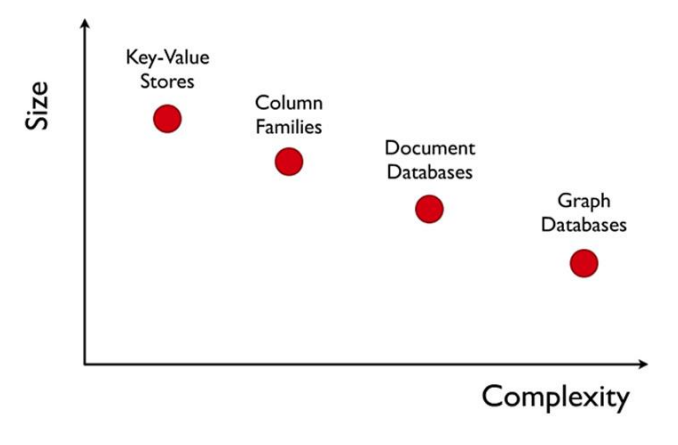
\includegraphics[scale=0.5]{./img/nosql/tipi_nosql.png}
      \caption{Tipi di database NoSQL}
      \label{fig:tipi_nosql}
      \centering
      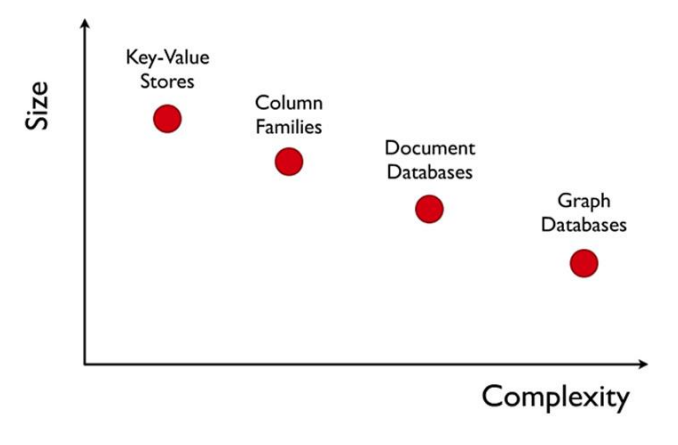
\includegraphics[scale=0.5]{./img/nosql/tipi_nosql.png}
      \caption{Tipi di database NoSQL}
      \label{fig:tipi_nosql}
\end{figure}

Rispetto questa rappresentazione possiamo posizionare il modello relazionale tra
il modello column-based e il modello document-based.


Rispetto questa rappresentazione possiamo posizionare il modello relazionale tra
il modello column-based e il modello document-based.

In questo corso vedremo i seguenti tipi di database NoSQL:
\begin{itemize}
      \item \textbf{Document-based}: i dati sono memorizzati in documenti, che
            possono essere in formato JSON, XML, BSON, YAML, etc.
      \item \textbf{Key-value}: i dati sono memorizzati in coppie chiave-valore.
      \item \textbf{Wide-column}: i dati sono memorizzati in colonne, simile ai
            database relazionali.
      \item \textbf{Graph-based}: i dati sono memorizzati in nodi e archi.
      \item \textbf{Document-based}: i dati sono memorizzati in documenti, che
            possono essere in formato JSON, XML, BSON, YAML, etc.
      \item \textbf{Key-value}: i dati sono memorizzati in coppie chiave-valore.
      \item \textbf{Wide-column}: i dati sono memorizzati in colonne, simile ai
            database relazionali.
      \item \textbf{Graph-based}: i dati sono memorizzati in nodi e archi.
\end{itemize}
Una caratteristica che accomuna queste tipologie di database è legata al problema
di mettere insieme i dati. Ad esempio, i database relazionali usano le operazioni
di join, mentre i database document-based usano un unico documento.
Una caratteristica che accomuna queste tipologie di database è legata al problema
di mettere insieme i dati. Ad esempio, i database relazionali usano le operazioni
di join, mentre i database document-based usano un unico documento.
\subsection{Key value}
I database \textbf{key-value} sono i più semplici tra i database NoSQL. In questi
I database \textbf{key-value} sono i più semplici tra i database NoSQL. In questi
database, i dati sono memorizzati come tabelle di hash dove la chiave punta a un
particolare valore. Si utilizzano le tabelle di hash per massimizzare le prestazioni
di lettura e scrittura.
\subsection{Wide column}
I database \textbf{wide-column} sono simili ai database relazionali, ma invece di
I database \textbf{wide-column} sono simili ai database relazionali, ma invece di
memorizzare i dati in righe, i dati sono memorizzati in colonne. Questo permette
di avere una maggiore flessibilità rispetto ai database relazionali. La chiave
punta a un insieme di colonne che può essere diverso per ogni riga.

\paragraph{HBASE}
HBase è un database wide-column che è stato ispirato da Google BigTable. In HBase
si ha una chiave che punta ad un insieme di valori che possono avere tipi differenti.

In questa struttura, possiamo definire delle \textbf{column family}, le quali
contengono più attributi che condividono delle informazioni. Il \textbf{qualifier} è
il nome dell'attributo all'interno di una column family. Ogni riga ha anche
un campo relativo al timestamp in cui è stata modificata.

L'utilizzo di timestamp fornisce un modo diverso per gestire le transazioni,
anche quelle distribuite, senza l'uso di lock. Questo metodo associa a ogni
transazione un timestamp, in modo che se due transazioni si sovrappongono,
possono essere risolte in base a tale valore.

In questa implementazione è possibile realizzare facilmente relazioni di tipo 1-n
nella stessa riga.
\paragraph{Cassandra}
Cassandra è un database wide-column che è stato realizzato da Facebook per gestire
la comunicazione con le mail.

Questo database si differenzia da HBase per il fatto si ha uno spazio delle chiavi,
il quale può essere visto come una tabella nel modello relazionale. Questo spazio
è suddiviso in column family, le quali sono differenti da quelle di HBase in quanto
la stessa chiave primaria può essere usata in più column family.

I valori che si trovano all'interno di una column family possono essere di tipo
diverso, inoltre, ogni riga ha un timestamp associato.

Quindi una column family equivale ad una \textit{tabella}, e si utilizza la chiave
primaria della riga per accedere ad un particolare dato di essa.

L'accesso viene effettuato specificando i seguenti campi:
\begin{itemize}
      \item \texttt{column family}
      \item \texttt{row key}
      \item \texttt{column name}
\end{itemize}
Per semplificare il passaggio da database relazionali a Cassandra, il query
language di Cassandra (CQL) è molto simile a SQL. Attraverso questo meccanismo
è possibile sviluppare un applicazione che è in grado di utilizzare sia database
relazionali che Cassandra senza apportare molte modifiche.

Un vantaggio dell'utilizzo di questo database è legato al fatto che ogni riga è
indipendente dalle altre. Quindi, in un contesto distribuito, è possibile frammentare
come si vuole il database senza dover fare join.

\paragraph{HBASE}
HBase è un database wide-column che è stato ispirato da Google BigTable. In HBase
si ha una chiave che punta ad un insieme di valori che possono avere tipi differenti.

In questa struttura, possiamo definire delle \textbf{column family}, le quali
contengono più attributi che condividono delle informazioni. Il \textbf{qualifier} è
il nome dell'attributo all'interno di una column family. Ogni riga ha anche
un campo relativo al timestamp in cui è stata modificata.

L'utilizzo di timestamp fornisce un modo diverso per gestire le transazioni,
anche quelle distribuite, senza l'uso di lock. Questo metodo associa a ogni
transazione un timestamp, in modo che se due transazioni si sovrappongono,
possono essere risolte in base a tale valore.

In questa implementazione è possibile realizzare facilmente relazioni di tipo 1-n
nella stessa riga.
\paragraph{Cassandra}
Cassandra è un database wide-column che è stato realizzato da Facebook per gestire
la comunicazione con le mail.

Questo database si differenzia da HBase per il fatto si ha uno spazio delle chiavi,
il quale può essere visto come una tabella nel modello relazionale. Questo spazio
è suddiviso in column family, le quali sono differenti da quelle di HBase in quanto
la stessa chiave primaria può essere usata in più column family.

I valori che si trovano all'interno di una column family possono essere di tipo
diverso, inoltre, ogni riga ha un timestamp associato.

Quindi una column family equivale ad una \textit{tabella}, e si utilizza la chiave
primaria della riga per accedere ad un particolare dato di essa.

L'accesso viene effettuato specificando i seguenti campi:
\begin{itemize}
      \item \texttt{column family}
      \item \texttt{row key}
      \item \texttt{column name}
\end{itemize}
Per semplificare il passaggio da database relazionali a Cassandra, il query
language di Cassandra (CQL) è molto simile a SQL. Attraverso questo meccanismo
è possibile sviluppare un applicazione che è in grado di utilizzare sia database
relazionali che Cassandra senza apportare molte modifiche.

Un vantaggio dell'utilizzo di questo database è legato al fatto che ogni riga è
indipendente dalle altre. Quindi, in un contesto distribuito, è possibile frammentare
come si vuole il database senza dover fare join.
\subsection{Document based}
I database \textbf{document-based} permettono di memorizzare delle informazioni sotto
forma di documenti. Ognuno dei quali è identificato attraverso una chiave unica.
Tutte le operazioni di lettura e manipolazione dei dati avvengono all'interno
dei documenti stessi.
\paragraph{MongoDB}
MongoDB è un database document-based che memorizza i dati in documenti JSON, più
precisamente, utilizza un formato binario di JSON chiamato BSON. Ogni documento
è identificato da una chiave unica, chiamata \texttt{\_id}.

Possiamo immaginare la struttura di un file JSON come un albero, dove la radice
è la chiave \texttt{\_id} e i figli sono i campi del documento.

Questa tipologia permette di salvare i dati come si faceva negli schemi relazionali,
ovvero suddividendo le informazioni in diverse \textbf{collezioni}. Per fare ciò,
si utilizzano i \textbf{riferimenti} tra i documenti. Lo svantaggio di questa
soluzione è che si devono fare molte join per ottenere l'informazione desiderata.

Un'altra soluzione è quella di salvare i dati in un unico documento, sfruttando
l'embedding, in modo da evitare le join. Questo metodo è molto efficiente quando
si devono accedere alle informazioni più vicine alla radice, ma meno efficiente
quando si devono accedere alle foglie, si ha comunque un tempo di accesso minore
rispetto alle join.

Nei database document-based lo schema non è vincolante, in particolare, corrisponde
all'unione di tutti gli attributi e sotto-attributi del documento.

Vediamo ora un parallelismo tra i database relazionali e MongoDB:
\begin{itemize}
      \item \textbf{Database} $\rightarrow$ \textbf{Database}
      \item \textbf{Tabella} $\rightarrow$ \textbf{Collection}
      \item \textbf{Row} $\rightarrow$ \textbf{Document}
      \item \textbf{Column} $\rightarrow$ \textbf{Field}
      \item \textbf{Index} $\rightarrow$ \textbf{Index}
      \item \textbf{Join} $\rightarrow$ \textbf{Embedded document}
      \item \textbf{Foreign key} $\rightarrow$ \textbf{Reference}
      \item \textbf{Partition} $\rightarrow$ \textbf{Shard}
\end{itemize}
Le operazioni che si vogliono svolgere sulla base di dati vengono espresse
attraverso una notazione che ricorda quella della programmazione a oggetti, ovvero
attraverso la \textit{dot notation}. Inoltre, nelle operazioni tutti gli
operatori devono essere espressi in JSON. Questo permette di eliminare l'utilizzo
di framework come Hibernate per mappare gli oggetti sul database.
\begin{nota}
      Quando si devono caricare grandi quantità di dati è utile disabilitare
      l'ack che viene mandato per ogni operazione.
\end{nota}
Le query di modifica di un documento presentano degli oggetti JSON come
clausole, simile alla clausola \texttt{WHERE} delle query SQL. Oltre a questo
è possibile specificare di creare un documento nuovo nel caso non sia presente
quello che si vuole modificare.

Mongo permette di creare degli indici per velocizzare le operazioni.
\begin{esempio}
      Vediamo ora un esempio di parallelismo tra una query SQL e una per
      MongoDB:
      \begin{center}
            db.\textcolor{red}{users}.find(\textcolor{green}{\{age: \{ \$gt: 18 \}\}},
            \textcolor{cyan}{\{name: 1, age: 1\}}).\textcolor{magenta}{limits(10)}
      \end{center}
      \begin{center}
            \textcolor{cyan}{SELECT name, age} \textcolor{red}{FROM users}
            \textcolor{green}{WHERE age $>$ 18} \textcolor{magenta}{LIMIT 10}
      \end{center}
\end{esempio}
Nelle interrogazioni, tutte le clausole sono specificate in \texttt{AND}, se si
vuole specificare in \texttt{OR} è necessario utilizzare il comando \$$or$ seguito
      da una lista di oggetti JSON.

      Nelle versioni successive è stato definito il concetto di \textbf{aggregation} e
      di \textbf{pipeline}. Una pipeline è un comando che rappresenta una sequenza di
      operazioni che vengono eseguite in serie e possono essere usate per operazioni
      di analytics.

      \begin{nota}
            Dato un problema non sempre per avere efficienza dobbiamo scegliere la
            soluzione banale, spesso dobbiamo prendere soluzioni controintuitive. Ex:
            salvare i dati non in modo efficiente e sfruttare la potenza di esecuzione
            delle query dei DBMS.
      \end{nota}
      \begin{nota}
            Un documento è un albero.
      \end{nota}
      \subsection{Graph based}
      I database graph-based memorizzano i dati salvando le informazioni nei nodi e
      utilizzando gli archi per definire delle relazioni tra esse. Questi database sono
      utili per memorizzare dati che hanno relazioni complesse, come ad esempio le
      relazioni dei social network.

      Spesso si usano per reti sociali, recommendations systems, logistica, financial
      transaction, bioinformatica, autorizzation and access control.

      I database basati sui grafi godono delle seguenti proprietà:
      \begin{itemize}
            \item \textbf{Storage}:
                  \begin{itemize}
                        \item \textbf{Nativo}: i dati vengono salvati sotto forma di
                              grafo, si ha la problematica legata alla scalabilità
                              della soluzione.
                        \item \textbf{Non nativo}: i dati vengono salvati in una struttura
                              differente da un grafo, ma che logicamente permette di essere
                              visto come un grafo.
                  \end{itemize}
            \item \textbf{Processing engine}:
                  \begin{itemize}
                        \item \textbf{Nativo}: permette di effettuare direttamente query
                              nel linguaggio dei grafi, sfruttando le proprietà dei
                              grafi. Il problema di questa soluzione è dovuto al fatto
                              che bisogna mappare le query reali utilizzando le proprietà
                              del grafo.
                        \item \textbf{Non nativo}: permette di utilizzare un altro
                              linguaggio (es. SQL) per effettuare query che non devono
                              per forza essere proprietà del grafo.
                  \end{itemize}
      \end{itemize}
      Lo storage nativo, spesso si basa sull'\textbf{index friend adjacency}, ovvero
      i nodi che sono vicini sono fisicamente salvati insieme. Questo permette di
      effettuare query molto velocemente, ma la costruzione del grafo è molto lenta.

      Il collegamento tra concetti si effettua attraverso un cammino tra nodi, mentre
      nel relazionale si effettua tramite valori, invece nel documentale si usa l'embedding.

      La struttura a grafo dei dati permette di rappresentare le informazioni
      attraverso un database documentale, ma essendo la base di tale modello una
      struttura ad albero risulta più complesso mappare le relazioni tra i dati.
      Per risolvere questo problema si utilizzando i riferimenti tra vari documenti.

      Un modo efficiente per modellare un grafo in modo non nativo è quello di sfruttare
      i vicini. Ad esempio, in un modello documentale possiamo utilizzare l'embedding
      per memorizzare i nodi vicini, mentre per i nodi lontani possiamo utilizzare i
      riferimenti.

      Una seconda soluzione è quella di usare relazioni differenti nel grafo per aumentare
      l'espressività del grafo e semplifica i collegamenti. Questo può essere implementato
      facilmente.

      \begin{esempio}
            Metti l'esempio del confronto delle interrogazioni tra modelli.
      \end{esempio}

      Nel modello a grafo, ogni nodo rappresenta le informazioni al suo interno con
      delle proprietà, ovvero coppie chiave-valore dove la chiave è rappresentata
      dall'etichetta e il valore rappresenta l'informazione. Anche le relazioni possono
      avere un etichetta a cui è associata una proprietà.

      Una stessa informazione può essere modellata in modi diversi, la scelta dipende
      dalle query che si vogliono effettuare. Le due soluzioni sono:
      \begin{itemize}
            \item \textbf{Stessa etichetta}: si ha una sola etichetta per accedere
                  a tutte le informazioni, mentre all'interno della relazione si specifica
                  il tipo di informazione.
            \item \textbf{Etichette multiple}: si ha una relazione per ogni tipo di
                  informazione.
      \end{itemize}
      Ad esempio, per modellare una situazione in cui a una persona sono associati più
      indirizzi, si possono utilizzare le due soluzioni, la scelta dipende dalle
      tipologie di query che si vogliono effettuare. Se si vogliono trovare tutti
      gli indirizzi di una persona, allora è meglio utilizzare una soluzione in cui
      si ha una stessa etichetta per accedere a tutti gli indirizzi e poi all'interno
      della relazione si specifica il tipo di indirizzo. Mentre, se si vogliono
      effettuare query per sapere uno specifico tipo di indirizzo è più conveniente
      utilizzare una relazione per ogni tipo di indirizzo.
      \paragraph{Query language}
      La modellazione tramite grafo risulta semplice a livello semantico da costruire,
      il problema è che non si ha uno standard per il Query language, eccone alcuni:
      \begin{itemize}
            \item \textbf{Cypher}: linguaggio dichiarativo basato sul \textbf{
                        pattern-matching query language} (come SQL), infatti
                  cerca tutti i sottografi che metchano con il grafo di query.
                  Permette di effettuare aggregation, ordering e limit.

                  Il risultato di una query grafo può essere una tabella o un
                  sottografo. La notazione di Cypher è la seguente:
                  \begin{center}
                        \texttt{(nodo)-[:etichetta]->(nodo2)}
                  \end{center}
                  Mettendo più condizioni separate dalla virgola equivale a
                  considerarle in and. Vediamo ora un esempio di query in Cypher:
                  \begin{lstlisting}[language=SQL]
                        MATCH (n:Person)-[r:KNOWS]->(m:Person)
                        WHERE n.name = 'Alice'
                        RETURN m.name
                  \end{lstlisting}
            \item \textbf{Gremlin} (graph traversal language): la query consiste
                  nel specificare un percorso. Il percorso viene inizializzato in
                  tutti i nodi. Nella query è possibile specificare dei constrain
                  su archi e nodi per selezionare quali percorsi considerare.

                  Questo linguaggio è pensato per essere eseguito ad agenti,
                  quindi è parallelizzabile ed eseguibile in ambienti distribuiti.

                  Vediamo un esempio di query in Gremlin:
                  \begin{lstlisting}[language=SQL]
                        g.V().has('name', 'Marko').out('KNOWS').values('name')
                  \end{lstlisting}
      \end{itemize}

      \section{Modelli poliglotti}
      Esistono delle soluzioni che integrano più modelli di database in un unico
      sistema, queste soluzioni sono chiamate modelli poliglotti.

      Un esempio di modello poliglotta è \textbf{ArangoDB}, un DBMS che supporta i
      seguenti modelli:
      \begin{itemize}
            \item \textbf{keyvalue}
            \item \textbf{graph}
            \item \textbf{document}
            \item \textbf{ricerca full text}
      \end{itemize}
      Tutti i modelli sono gestiti come documenti JSON, più precisamente si hanno due
      documenti principali:
      \begin{itemize}
            \item \textbf{databases} (schemas): contengono lo schema generico delle collections
            \item \textbf{collections} (tables): contengono documenti JSON di tipi simili
      \end{itemize}
      In questo modo si possono facilmente gestire i modelli key-value. Per quanto riguarda
      il graph model, in questo caso ArangoDB utilizza una collection per specificare
      i nodi, ciascun nodo viene descritto da un documento JSON. Successivamente si
      rappresentano i collegamenti utilizzando una nuova collection che contiene un documento
      JSON per ogni arco. Il documento contiene gli indici dei due nodi e quindi si effettua
      il referencing tra documenti. In fase di query si effettuerà la Join per collegare
      i nodi agli archi.
      \section{Distribuited NoSQL}
      I sistemi RDBMS sono facilmente scalabili verticalmente (\textbf{Scale up}),
      ovvero si potenzia la singola macchina, ma non sono facilmente scalabili
      orizzontalmente (\textbf{scale out}), il che consiste nell'aggiungere nodi
      all'infinito al cluster.

      Questo vincolo è dovuto alle proprietà ACID che devono essere rispettate per
      definizione. Questo non è un problema per i database NoSQL, in quanto sono
      progettati per essere scalati orizzontalmente. Infatti, per questi database vale
      il CAP theorem, il quale afferma che:
      \begin{teorema}[\textbf{CAP theorem}]
            In un sistema distribuito non è possibile garantire contemporaneamente
            le tre proprietà seguenti:
            \begin{itemize}
                  \item \textbf{Consistency}: tutti i nodi vedono gli stessi dati
                  \item \textbf{Availability}: ogni richiesta riceve una risposta
                  \item \textbf{Partition tolerance}: il sistema continua a funzionare
                        anche in presenza di partizioni di rete
            \end{itemize}
            al massimo due di queste proprietà possono essere garantite contemporaneamente.
      \end{teorema}
      Con la nuova scoperta si ogni DBMS si è incentrato su solo 2 proprietà di quelle
      descritte. Generalmente i RDBMS rispettano CA, mentre per i NoSQL, per via delle
      proprietà BASE, non si limitano alla combinazione di solo CA. Con queste considerazioni
      i sistemi NoSQL sono più facili da scalare (vedi figura \ref{fig:cap}).
      \begin{figure} [!ht]
            \centering
            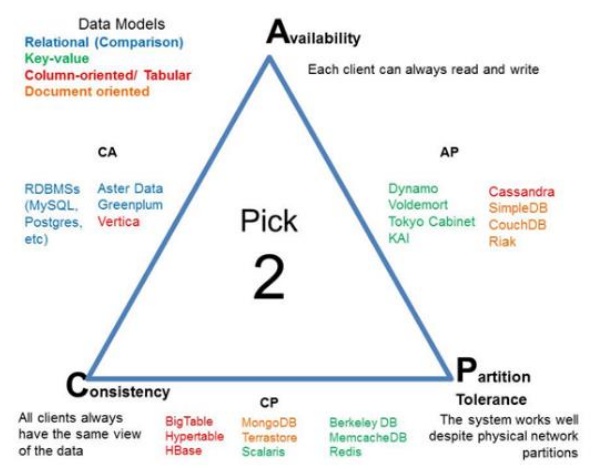
\includegraphics[width=0.5\textwidth]{img/nosql/CAP.png}
            \caption{DBMS con le proprietà che assicurano di rispettare}
            \label{fig:cap}
      \end{figure}
      Oltre a questo teorema, i modelli NoSQL si basano sul principio \textbf{BASE},
      ovvero:
      \begin{itemize}
            \item \textbf{Basically Available}: il sistema garantisce una disponibilità
                  di servizio anche in presenza di fallimenti
            \item \textbf{Soft state}: lo stato del sistema può cambiare anche in assenza
                  di input
            \item \textbf{Eventually consistent}: il sistema raggiunge uno stato consistente
                  in un certo momento, anche se non è garantito che lo sia in ogni momento
      \end{itemize}
      \subsection{Keyvalue model: Redis}
      Redis essengo un keyvalue non effettua frammentazione, permette di creare dei
      cluster con più nodi e permette di implementare meccanismi automatici e trasparenti
      di replica per avere alta Availability.

      La replica può essere implementata a livello di cluster, si utilizza un cluster
      "Master" di nodi su cui si effettuano le letture e le scritture, successivamente
      si utilizzano dei cluster "Slave" di nodi su cui si effettua la replica dei cluster
      "Master", questi vengono usati principalmente in lettura. Un'altra implementazione
      è tramite la definizione delle repliche sugli stessi nodi del cluster, questo
      comporta che non abbiamo meccanismi Master-slave a livello di cluster, bensì a
      livello di nodi. Quindi per ogni cluster possiamo sia leggere sia scrivere
      (vedi \ref{fig:dist_redis}).
      \begin{figure} [!ht]
            \centering
            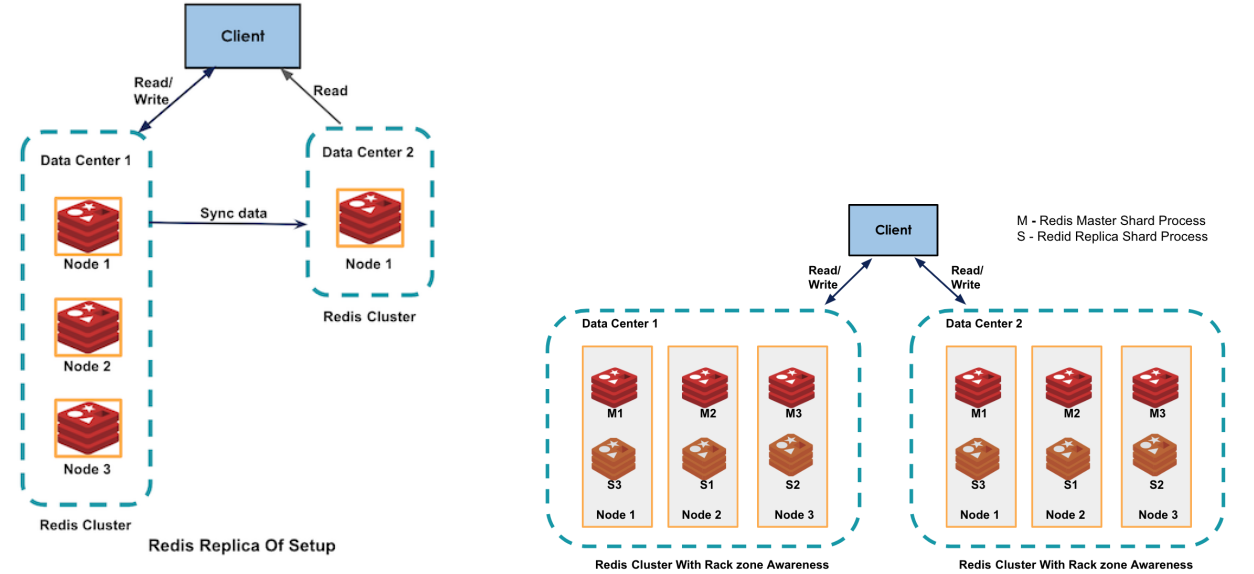
\includegraphics[width=0.5\textwidth]{img/nosql/redis_distribuited.png}
            \caption{Due metodologie per replicare con Redis}
            \label{fig:dist_redis}
      \end{figure}

      Le shard create possono essere:
      \begin{itemize}
            \item \textbf{Dense}: se un nodo ha abbastanza memoria allocata per il
                  database, allora le shard possono essere posizionate sullo stesso nodo
                  e solamente dopo che è pieno si passa a un nuovo nodo.
            \item \textbf{Sparse}: viene utilizzato il massimo numero di nodi per
                  distribuire le shard.
      \end{itemize}
      \subsection{Column Family model: HBASE}
      La distribuzione con HBase si basa sul meccanismo Master-slave e sulla frammentazione
      orizzontale, ciascun frammento si chiama \textbf{Region}.

      La distribuzione si basa su 2 componenti:
      \begin{itemize}
            \item \textbf{HBase master}: è un'istanza di HBase che si occupa di
                  coordinare gli slave, assegna i region agli slave e riconosce i
                  fallimenti. Permette inoltre di effettuare operazioni di admin.
            \item \textbf{Region server}: sono le singole istanze slaves del cluster,
                  si occumano di salvare effettivamente i region assegnati dal master
                  e si occupa di gestirli, fornisce le funzioni di lettura e scrittura
                  dei suoi region tramite i log. Su ogni Region server si possono
                  implementare meccanismi di replica.
            \item \textbf{Hbase Client}: è il client che dialoga con il master per fare le
                  richieste.
      \end{itemize}
      Il cluster sarà formato da un nodo HBase master e tanti Region Server, quest'ultimi
      possono avere diversi nodi per la replica. Nel cluster si avrà poi un'orchestratore
      (\textbf{ZooKeeper}) che permette il coordinamento tra Client, Master e Slaves
      in modo da risolvere eventuali problemi di fallimento (vedi \ref{fig:dist_hbase})
      \begin{figure} [!ht]
            \centering
            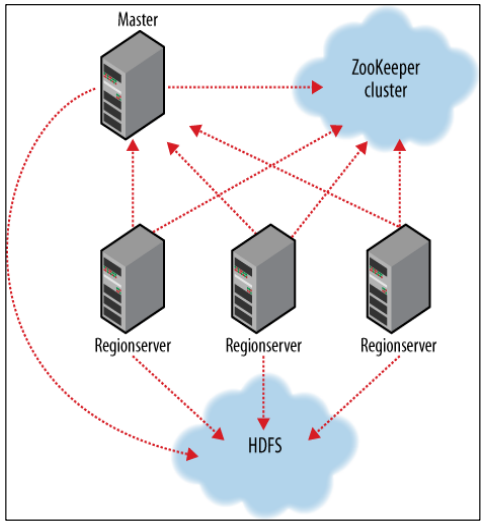
\includegraphics[width=0.4\textwidth]{img/nosql/hbase_distribuited.png}
            \caption{Architettura distribuita HBase}
            \label{fig:dist_hbase}
      \end{figure}
      \subsection{Column Family model: CASSANDRA}
      Cassandra distribuito ha un'architettura a cluster, ciascuno viene gestito in peer
      to peer con una rete ad anello. I dati vengono partizionati tra in nodi della rete e
      per risolvere i fallimenti si usa la replicaizone. Si scrive e legge su qualsiasi
      nodo, il numero di nodi del cluster può essere aggiornato a runtime.

      Le performance dipendono linearmente rispetto al numero di nodi.

      Essendo un'architettura peer-to-peer allora non ha single point of failure
      fornendo massima Availability. In aggiunta si può partizionare il database
      su più cluster differenti e separati geograficamente.

      Cassandra implementa anche la replicazione dei dati di un cluster in due modi:
      \begin{itemize}
            \item \textbf{Replicazione su un nodo}: si replicano i dati sullo
                  stesso nodo
            \item \textbf{Replicazione su un nodo diverso}: si replicano i dati su un
                  altro nodo dello stesso cluster. Questo permette di salvarsi dalla
                  perdita di dati se un nodo si guasta perché ci sarà una replica in
                  un altro nodo.
      \end{itemize}
      Si utilizzerà zookeeper per gestire le repliche, nota che le repliche devono essere
      almento $3$.

      Ogni cluster gestisce una partizione del database. Ognuna di queste presenta
      un ulteriore partizionamento dei dati, il quale viene gestito dai nodi interni.

      Il partizionamento avviene sfruttando funzioni di hashing. I nodi sono divisi in
      modo logico in una forma ad anello, detta ring topology. Si usano quindi i valori
      hash delle chiavi, associate alle partizioni dati, per assegnare l'informazione
      a uno dei nodi.

      Ciascun nodo viene posizionato nell'anello e gli viene associato un particolare
      valore, in questo modo ciascun nodo si occupa dei dati le cui funzioni di hash
      mappano l'informazione nella porzione di anello che va dal nodo precedente al
      nodo stesso.

      Quando si aggiunge un nuovo nodo si divide lo spazio di indirizzamento in modo
      da avere una distribuzione uniforme e i dati vengono replicati in modo automatico.

      Dal momento che si ha un'architettura peer-to-peer, per comunicare lo stato
      dei nodi e la locazione dei dati nel cluster si usa il \textbf{gossip protocol}.
      Questo protocollo permette di comunicare in modo efficiente tra i nodi, sfruttando
      il seguente meccanismo: se i dati non sono sul nodo attuale, allora si chiede a
      quelli adiacienti, i quali a loro volta controllano se hanno le informazioni. In
      caso contrario chiedono a quelli adiacienti, fino a quando non sono stati visitati
      tutti i nodi.

      Utilizzando il \textbf{gossip protocol} si può facilemnte \textbf{identificare
            il fallimento}, infatti, ogni nodo tiene salvato la sua probabilità di
      fallimento e in fase di comunicazione, in base alla velocità delle risposte
      aggiorna la sua probabilità, in questo modo si aumenta quando le condizioni
      della rete peggiorano, come la latenza ecc\dots

      Si usa una soglia che specifica sopra quanto la probabilità deve essere per considerare
      il nodo dead. Non si usa una politica basata sui timeout in quanto la rete può
      essere riempita di messaggi di gossip e quindi si può avere un ritardo.

      Le operazioni di scrittura su ciascun nodo seguono questi passi:
      \begin{itemize}
            \item Scrivo l'operazione nel LOG
            \item Scrivo il dato in RAM
            \item Quando i dati in RAM sono abbastanza scrivo su disco
      \end{itemize}

      Dal momento che si hanno partizioni e repliche in un particolare cluster, diventa
      fondamentale gestire la consistenza, in fase di query si deve specificare
      la tipologia di consistenza e il replication\_factor e successivamente in base
      alle operazioni si hanno diversi livelli di consistenza:
      \begin{itemize}
            \item scrittura:
                  \begin{itemize}
                        \item consistency one: si ritorna la risposta al client dopo una scrittura
                              su disco solo su un nodo del cluster
                        \item consistency all: si ritorna la risposta al client dopo una scrittura
                              su disco solo su un numero di nodi del cluster pari al replication factor
                        \item consistency quorum: si ritorna la risposta al client dopo $replication\_factor/2+1$ nodi che
                              hanno scritto su disco
                  \end{itemize}
            \item lettura:
                  \begin{itemize}
                        \item consistency one: si ritorna la risposta al client dopo la lettura
                              su un nodo del cluster
                        \item consistency all: si ritorna la risposta al client dopo una lettura
                              solo su un numero di nodi del cluster pari al replication factor
                  \end{itemize}
      \end{itemize}

      Le query di cancellazione vengono implementate attraverso le marcature che
      comunicano che il record è cancellato ma lo cancellano effettivamente in un secondo
      momento, più precisamente attraverso \textbf{major compaction} o dopo un timer.

      In merito alle operazioni di delete si ha che esse semplicemente rendono il
      dato non disponibile, essendo più veloce cambiare un flag piuttosto che cancellare.
      A causa di ciò comunque si creano nelle tabelle fisiche dei problemi di
      spazio, quindi periodicamente si fanno dei merge, ovvero ogni singolo nodo
      procede alla “compattazione” dei propri dati, sovrascrivendo i valori non più
      disponibili.

      Per assicurare la sincronizzazione dei nodi e per evitare perdita di consistenza
      si utilizzano dei checksum per comparare i dati di un nodo con quelli dei
      successivi. Per effettuare questo controllo, nel dettaglio, vengono usati degli
      hash-tree detti \textbf{Merkle tree} nel seguente modo:
      \begin{itemize}
            \item Vengono mandati degli snapshot dei dati ai nodi successivi.
            \item Vengono creati e trasmessi ad ogni “compattazione” principale.
            \item Se due nodi prendono uno snapshot con un intervallo pari a
                  \texttt{TREE\_STORE\_TIMEOUT} allora i due snapshot sono comparati e in
                  caso di successo i dati vengono sincronizzati.
      \end{itemize}
      Cassandra rientra nella catergoria AP.
      \subsection{Document model: MongoDB}
      MongoDB ha un'architettura master (primary) e slave (secondary). Si effettuano le
      scritture sul primary che poi replica sui secondary usando il file di LOG del primary.

      In sostanza ciascun cluster di nodi è chiamato shard, in ogni shard si identifica
      un nodo primary e tutti gli altri saranno secondary. Se il primary dovesse cadere
      allora si effettuerà un'elezione tra i secondary per identificare il nuovo primary,
      l'elezione si baserà sui nodi che sono più aggiornati e in questa fase le
      scritture si interrompono.

      Per identificare quando un nodo dello shard cade si effettua un heartbeat con timeout
      per avvisare gli altri che sono attivi, nel replica set si ha una gerarchia dei
      nodi, ogni nodo ha un numero che specifica il livello di priorità. In caso il
      primary cade allora il secondary con la priorità più alta chiede le elezioni.
      Ne replica set si possono avere al massimo 50 nodi di cui $7$ solo votanti.

Un nodo può essere definito:
\begin{itemize}
      \item votante: può lasciare un solo voto
      \item non votante: deve avere priorità a $0$
\end{itemize}

La frammentazione dei dati avviene separando i dati tra i vari shard.

L'architettura distribuita si basa su 3 componenti:
\begin{itemize}
      \item mongos: è il punto di accesso software per le query, tutte le query
            verranno eseguite su questo processo. Quando riceve una query capisce
            dove sono i frammenti, grazie al config server, e quindi procede con
            la query di tipo:
            \begin{itemize}
                  \item target query se deve interrogare solo un nodo
                  \item broadcast query se deve interrogare più nodi
            \end{itemize}
      \item config server: ovvero un file che conosce la struttura degli shard,
            conoscendo frammentazioni e repliche.
      \item Shards: singoli cluster che salvano un frammento dei dati.
\end{itemize}
La scrittura avviene sul nodo primario e si hanno diverse politiche in base
tramite l'opzione writeConcern che dice cosa fare per le replicaSet. Si hanno
tre parametri:
\begin{itemize}
      \item w: indica il numero di nodi in cui il dato deve essere replicato
            prima di essere considerata conclusa l'operazione. Nel dettaglio,
            possiamo avere:
            \begin{itemize}
                  \item w = 0: non da alcuna certezza di inserimento, utile per
                        operazioni veloci
                  \item w = 1: implica la scrittura sul nodo primary
                  \item w = n: implica la scrittura su n nodi
                  \item w = majority: dove almeno la metà dei nodi più 1 deve aver
                        scritto prima della conferma dell'operazione
            \end{itemize}
      \item j: ovvero l'intenzione di scrivere sul log di Wiredtiger, tramite la
            logica write ahead logging.
      \item wtimeout: ovvero il tempo limite, espresso in ms, da aspettare nel
            caso in cui $w > 0$, se 0 non devo aspettare risposta da nessuno.
\end{itemize}
Per quanto riguarda le letture, si utilizza una politica di readConcern, la quale
deve essere consistente come per writeConcern, facendo scegliere se è più
dispendioso scrivere o leggere:
\begin{itemize}
      \item local: è il valore di default per leggere i dati dai nodi in un
            replicaSet. La query è fatta secondo la località spaziale e quindi
            se legge un nodo non primary rischio di leggere dati non ancora
            replicati.
      \item available: di default per lettura su nodi secondari, che fa vedere
            che il dato c'è ed è consistente.
      \item majority: quando almeno metà più 1 repliche ha ricevuto un ack
            in scrittura sul dato allora posso leggere.
\end{itemize}
Dalla versione 4.0 MongoDB ha introdotto nel modello documentale le transazione
tramite l'engine Wiredtiger. Introduce quindi il concetto di log che indica che
tutto è nel nodo primary. Si opera sempre sul nodo facendo un lock che può essere
di tipo:
\begin{itemize}
      \item shared (S): per le letture
      \item exclusive (X): per le scritture
      \item intent sharded (IS): esprimere l'intenzione di bloccare in
            modo condiviso uno dei nodi che discende dal nodo corrente.
      \item intent exclusive (IX): per esprimere l'intenzione di bloccare in
            modo esclusivo uno dei nodi che discende da quello corrente:
\end{itemize}

Mongo rientra nella catergoria CP.


\end{document}